% Arquivo LaTeX de exemplo de dissertação/tese a ser apresentados à CPG do IME-USP
% 
% Versão 5: Sex Mar  9 18:05:40 BRT 2012
%
% Criação: Jesús P. Mena-Chalco
% Revisão: Fabio Kon e Paulo Feofiloff
%  
% Obs: Leia previamente o texto do arquivo README.txt

\documentclass[11pt,twoside,a4paper]{book}

% ---------------------------------------------------------------------------- %
% Pacotes 

\usepackage[utf8]{inputenc}
\usepackage[T1]{fontenc}
\usepackage{graphicx}           % usamos arquivos pdf/png como figuras
%\usepackage{setspace}                   % espaçamento flexível
\usepackage{indentfirst}                % indentação do primeiro parágrafo
\usepackage{makeidx}                    % índice remissivo
\usepackage[nottoc]{tocbibind}          % acrescentamos a bibliografia/indice/conteudo no Table of Contents
\usepackage{courier}                    % usa o Adobe Courier no lugar de Computer Modern Typewriter
\usepackage{fix-cm}                    % fontes realmente escaláveis
\usepackage{listings}                   % para formatar código-fonte (ex. em Java)
\usepackage{titletoc}
%\usepackage[bf,small,compact]{titlesec} % cabeçalhos dos títulos: menores e compactos
%\usepackage[fixlanguage]{babelbib}
\usepackage[font=small,format=plain,labelfont=bf,up,textfont=it,up]{caption}
\usepackage[usenames,svgnames,dvipsnames]{xcolor}
\usepackage[a4paper,top=2.54cm,bottom=2.0cm,left=2.0cm,right=2.54cm,headheight=23pt]{geometry} % margens
%\usepackage[pdftex,plainpages=false,pdfpagelabels,pagebackref,colorlinks=true,citecolor=black,linkcolor=black,urlcolor=black,filecolor=black,bookmarksopen=true]{hyperref} % links em preto
\usepackage[square,sort,nonamebreak,comma]{natbib}  % citação bibliográfica alpha (alpha-ime.bst)
\fontsize{60}{62}\usefont{OT1}{cmr}{m}{n}{\selectfont}

% ---------------------------------------------------------------------------- %
% Cabeçalhos similares ao TAOCP de Donald E. Knuth
\usepackage{fancyhdr}
\pagestyle{fancy}
\fancyhf{}
\renewcommand{\chaptermark}[1]{\markboth{\MakeUppercase{#1}}{}}
\renewcommand{\sectionmark}[1]{\markright{\MakeUppercase{#1}}{}}
\renewcommand{\headrulewidth}{0pt}

\usepackage{setspace}
\usepackage{multirow}
\usepackage{array}
\usepackage{import}
\usepackage{tikz}
\usepackage{colortbl}
\usepackage{tabularx}
\usepackage{flushend}
\usepackage{amsmath}
\usepackage{epstopdf}
\usepackage{float}
\usepackage{xcolor,colortbl}
\usepackage{subcaption}
\usepackage{keyval,xparse}
\mathchardef\mhyphen="2D
\usepackage[stable,perpage,flushmargin]{footmisc}

%load hyperref last
\usepackage[pdftex,plainpages=false,pdfpagelabels,pagebackref,colorlinks=true,citecolor=DarkGreen,linkcolor=NavyBlue,urlcolor=DarkRed,filecolor=green,bookmarksopen=true,bookmarks=false]{hyperref} % links coloridos

%esciece15
\newcommand{\joinNameTweet}[2] {
\texttt{\textbf{#1:} #2}
}

\newcommand{\tweetRowFull}[4] {
\stepcounter{rowcount}
\multirow{2}{0.3cm}{ \therowcount }	& 
\multirow{2}{0.7cm}{ $#2$ } 	& 
#3 \\
&& 
\cellcolor{gray!25} #4 \\ \cline{1-3}
}

\newcommand{\tweetTableFull}[5] {
%\onecolumn
\newcounter{rowcount}
\setcounter{rowcount}{0}
\begin{table*}[!htbp]
	\centering
	%\footnotesize
	\fontsize{6.5pt}{7pt}\selectfont
		\caption{#1}
		%\hspace*{-0.5cm}  
		\setlength\tabcolsep{0.05cm}
		\begin{tabularx}{\linewidth}{|>{\raggedright\arraybackslash}m{0.3cm}|>{\raggedright\arraybackslash}m{0.7cm}|>{\raggedright\arraybackslash}m{16.5cm}|}
			\cline{1-3}
			\centering\arraybackslash \textbf{\#} & \centering\arraybackslash \textbf{Score} & \centering\arraybackslash \textbf{Retweets} \\ \cline{1-3} 
			\input{#3}
			\multicolumn{3}{l}{}\\ \cline{1-3}
			\centering\arraybackslash \textbf{\#} & \centering\arraybackslash \textbf{Score} & \centering\arraybackslash \textbf{Replies} \\ \cline{1-3} 
			\input{#4}
			\multicolumn{3}{l}{}\\ \cline{1-3}
			\centering\arraybackslash \textbf{\#} & \centering\arraybackslash \textbf{Score} & \centering\arraybackslash \textbf{Non-Tagged} \\ \cline{1-3} 
			\input{#5}
		\end{tabularx}
	\label{tab:#2}
\end{table*}
%\twocolumn
}

%\newcommand{\tweetRow}[3] {
			%\multirow{2}{*}{
			%#1
			%} & \multicolumn{1}{|p{6cm}|}{\texttt{
			%#2
			%}} \\ \cline{2-2} & \multicolumn{1}{|p{6cm}|}{\texttt{
			%#3
			%}} \\ \hline
			%}
			
%\newcommand{\tweetTable}[3] {
%\begin{table}[!htbp]
	%\centering
	%\scriptsize
		%\caption{#3}
		%\begin{tabular}{|m{1.75cm}l}
			%\hline
			%\multicolumn{2}{|c|}{#3} \\ \hline
			%\input{C:/sam/Dropbox/Usp/phd/repo/egonet/pictures/lost_behavior/#1/#2/input_#3_all_but_replies_retweets}
		%\end{tabular}
	%\label{tab:#3}
%\end{table}
			%}
		


%www16
\makeatletter
\define@key{subimagedic}{width}{\def\width{#1}}
\define@key{subimagedic}{scale}{\def\scale{#1}}
\makeatother
\NewDocumentCommand\subimage{O{} m G{}}{
    \begingroup
        \setkeys{subimagedic}{width={1.0},scale={1.0}, #1}
        \begin{subfigure}{\width\textwidth}
            \expandafter\includegraphics\expandafter[scale=\scale]{#2}
        \caption{#3}\end{subfigure}
    \endgroup
}

% ---------------------------------------------------------------------------- %
\frenchspacing                          % arruma o espaço: id est (i.e.) e exempli gratia (e.g.) 
\urlstyle{same}                         % URL com o mesmo estilo do texto e não mono-spaced
\makeindex                              % para o índice remissivo
\raggedbottom                           % para não permitir espaços extra no texto
\fontsize{60}{62}\usefont{OT1}{cmr}{m}{n}{\selectfont}
\cleardoublepage
\normalsize

% ---------------------------------------------------------------------------- %
% Opções de listing usados para o código fonte
% Ref: http://en.wikibooks.org/wiki/LaTeX/Packages/Listings
\lstset{ %
language=Java,                  % choose the language of the code
basicstyle=\footnotesize,       % the size of the fonts that are used for the code
numbers=left,                   % where to put the line-numbers
numberstyle=\footnotesize,      % the size of the fonts that are used for the line-numbers
stepnumber=1,                   % the step between two line-numbers. If it's 1 each line will be numbered
numbersep=5pt,                  % how far the line-numbers are from the code
showspaces=false,               % show spaces adding particular underscores
showstringspaces=false,         % underline spaces within strings
showtabs=false,                 % show tabs within strings adding particular underscores
frame=single,                    % adds a frame around the code
framerule=0.6pt,
tabsize=2,                        % sets default tabsize to 2 spaces
captionpos=b,                   % sets the caption-position to bottom
breaklines=true,                % sets automatic line breaking
breakatwhitespace=false,        % sets if automatic breaks should only happen at whitespace
escapeinside={\%*}{*)},         % if you want to add a comment within your code
backgroundcolor=\color[rgb]{1.0,1.0,1.0}, % choose the background color.
rulecolor=\color[rgb]{0.8,0.8,0.8},
extendedchars=true,
xleftmargin=10pt,
xrightmargin=10pt,
framexleftmargin=10pt,
framexrightmargin=10pt
}

% ---------------------------------------------------------------------------- %
% Corpo do texto
\begin{document}
\hypersetup{pageanchor=false}
\frontmatter
% cabeçalho para as páginas das seções anteriores ao capítulo 1 (frontmatter)
\fancyhead[RO]{{\footnotesize\rightmark}\hspace{2em}\thepage}
\setcounter{tocdepth}{2}
\fancyhead[LE]{\thepage\hspace{2em}\footnotesize{\leftmark}}
\fancyhead[RE,LO]{}
\fancyhead[RO]{{\footnotesize\rightmark}\hspace{2em}\thepage}

\onehalfspacing  % espaçamento

% ---------------------------------------------------------------------------- %
% CAPA
% Nota: O título para as dissertações/teses do IME-USP devem caber em um 
% orifício de 10,7cm de largura x 6,0cm de altura que há na capa fornecida pela SPG.
\thispagestyle{empty}
\begin{center}
    \vspace*{2.3cm}
    \textbf{\Large{\phdTitle}}\\
    
    \vspace*{1.2cm}
    \Large{Samuel Martins Barbosa Neto}
    
    \vskip 2cm
    \textsc{
    Thesis presented\\[-0.25cm] 
    to the\\[-0.25cm]
    Institute of Mathematics and Statistics\\[-0.25cm]
    of the\\[-0.25cm]
    University of São Paulo\\[-0.25cm]
    as requirement\\[-0.25cm]
    to obtain the title\\[-0.25cm]
    of\\[-0.25cm]
    Doctor of Philosophy}
    
    \vskip 1.5cm
    Program: Computer Science\\
    Advisor: Prof. Dr. Roberto Marcondes Cesar Jr.\\
    Coadvisor: Dr. Claudio Santos Pinhanez \\
    Foreign Advisor: Prof. Dr. Dan Cosley

       \vskip 1cm
    \normalsize{The author received financial support from CAPES/CNPq/FAPESP}
    
    \vskip 0.5cm
    \normalsize{São Paulo, \finalMonth~\thesisYear}
\end{center}

% ---------------------------------------------------------------------------- %
% Página de rosto (Só PARA A VERSãO DEPOSITADA - ANTES DA DEFESA)
% Resolução CoPGr 5890 (20/12/2010)
%
% IMPORTANTE:
%   Coloque um '%' em todas as linhas
%   desta página antes de compilar a versão
%   final, corrigida, do trabalho
%
%
\newpage
\thispagestyle{empty}
    \begin{center}
        \vspace*{2.3 cm}
        \textbf{\Large{\phdTitle}}\\
        \vspace*{2 cm}
    \end{center}

    \vskip 2cm

    \begin{flushright}
    This is the original version of the thesis written by the\\
    candidate (Samuel Martins Barbosa Neto), as\\
    submitted to the Judging Committee.
    \end{flushright}

\pagebreak


 %---------------------------------------------------------------------------- %
 %Página de rosto (Só PARA A VERSãO CORRIGIDA - APóS DEFESA)
 %Resolução CoPGr 5890 (20/12/2010)
%
 %Nota: O título para as dissertações/teses do IME-USP devem caber em um 
 %orifício de 10,7cm de largura x 6,0cm de altura que há na capa fornecida pela SPG.
%
 %IMPORTANTE:
   %Coloque um '%' em todas as linhas desta
   %página antes de compilar a versão do trabalho que será entregue
   %à Comissão Julgadora antes da defesa
%
%
\newpage
\thispagestyle{empty}
    \begin{center}
        \vspace*{2.3 cm}
        \textbf{\Large{\phdTitle}}\\
        \vspace*{2 cm}
    \end{center}

    \vskip 2cm

    \begin{flushright}
    This version of the thesis contains the corrections and suggestions given by\\
    the Judging Committee during the defense of the original version of the work,\\
    that took place on \thesisMonth~\thesisDay, \thesisYear. A copy of the original version is available at the\\
    Institute of Mathematics and Statistics of the
University of São Paulo.

    \vskip 2cm

    \end{flushright}
    \vskip 4.2cm

    \begin{quote}
    \noindent Judging Committee:
    
    \begin{itemize}
        \item Prof. Dr. Roberto Marcondes Cesar Junior --- IME --- USP
        \item Dr. Claudio Santos Pinhanez --- IBM Research Brazil
        \item Prof. Dr. Denis Deratani Mauá --- IME --- USP
        \item Prof. Dr. Jesus Mena---Chalco --- UFABC
        \item Prof. Dr. Luciano Digiampietri --- EACH --- USP
    \end{itemize}
      
    \end{quote}
\pagebreak


\pagenumbering{roman}     % começamos a numerar 

% ---------------------------------------------------------------------------- %
% Agradecimentos:
% Se o candidato não quer fazer agradecimentos, deve simplesmente eliminar esta página 
\chapter*{Acknowledgements}

This thesis came to be in great part due to the efforts and support of Dan Cosley, to whom I am greatly thankful. The discussions and contributions of Amit Sharma were also very much appreciated. This was a 5-year journey, which I dedicate to family and friends, all those who made it so enjoyable. Far too many people provided precious contributions in the most varied ways, some are still around while others drifted away, but in thought I will cherish all the moments that led to this conclusion.


% ---------------------------------------------------------------------------- %
% Resumo
\chapter*{Resumo}

\noindent \surnameAbbr~\textbf{\phdTitleBr}. 
\thesisYear. \thesisPages f. Tese (Doutorado) - Instituto de Matemática e Estatística,
Universidade de São Paulo, São Paulo, \thesisYear.
\\

Comunidades online proporcionam um ambiente fértil para a análise do comportamento de indivíduos e avanços na compreensão de processos sociais. Por exemplo, quando modelamos interações sociais online, é importante compreender quando indivíduos estão reagindo a outros indivíduos. Além disso, pessoas e comunidades mudam com o passar do tempo, e nós argumentamos que análises de comunidades online que levam em consideração a evolução temporal fornecem resultados mais precisos e profundos. Entretanto, em muitos casos, o comportamento de usuários pode facilmente ser perdido: muitas das reações dos usuários ao conteúdo que são expostos não são capturadas por indicadores explicitos (como \textsl{likes} no Facebook ou \textit{replies} no Twitter). Aggregações temporais de dados pouco criteriosas podem ocultar, enviesar ou mesmo levar a conclusões equivocadas sobre a forma como os usuários evoluem. 

Para tratar o problema de detectar respostas não-explicitas, nós apresentamos uma nova abordagem que utiliza a similaridade medida por tf-idf entre os tweets de um usuário e os tweets recentes que este usuário recebeu das pessoas que ele segue. Nos baseando em dados de postagens de um mês para 449 redes egocêntricas no Twitter, este método evidencia que temos um provável volume de ao menos 11\% de reações que não são capturadas pelos mecanismos explicitos de \textit{reply} e \textit{retweet}. Mais do que isso, essas reações que não são capturadas não estão uniformemente distribuídas entre os usuários: alguns usuários que criam \textit{replies} e \textit{retweets} sem utilizar os mecanismos formais da interface são muito mais responsivos a quem eles seguem do que aparentam. Isso sugere que detecetar respostas não-explicitas é importante quando consideramos mitigar viéses e construir modelos mais precisos baseados nestes identificadores de respostas a fim de estudar iterações sociais e difusão de informação. 

Nós também abordamos o problema de evolução dos usuários no Reddit, nos baseando em dados de comentários e submissões no período de 2007 a 2014. Mesmo utilizando um dos métodos mais simples de diferenciação temporal dos usuários-cohorts anuais-nós encontramos amplas diferenças entre o comportamento dos indivíduos, que incluem criação de comentários, métricas de esforço e sobrevivência. Além disso, não considerar a evolução temporal pode levar a equívocos a repeito de fenômenos importantes. Por exemplo, uma de nosssas observações é que o tamanho médio dos comentários na rede decresce ao longo de qualquer intervalo de tempo arbitrário, mas o tamanho médio dos comentários em cada uma das cohorts de usuários é crescente no mesmo intervalo de tempo, salvo de uma queda inicial, que caracteriza uma observação do Paradoxo de Simpson. Dividindo as cohorts de usuários em sub-cohorts baseadas em anos de sobrevivência na rede nos fornece uma perspectiva melhor;  usuários que sobrevivem por mais tempo apresentam um maior nível de atividade inicial, fazendo mais comentários mais curtos do que aqueles usuários que sobrevivem menos. Estes elementos nos fornecem uma compreensão melhor de como usuários no Reddit evoluem e levantam uma série de questões interessantes a respeito de futuros desdobramentos do estudo de comportamento online.
\\

\noindent \textbf{Palavras-chave:} comportamento de usuários, redes sociais, reações, paradoxo de simpson, twitter, reddit.

% ---------------------------------------------------------------------------- %
% Abstract
\chapter*{Abstract}
\noindent \surnameAbbr~\textbf{\phdTitle}.
\thesisYear. \thesisPages p. Thesis (Ph.D.) - Institute of Mathematics and Statistics,
University of São Paulo, São Paulo, \thesisYear.
\\


Online communities provide a fertile ground for analyzing people’s behavior and improving our understanding of social processes. For instance, when modeling social interaction online, it is important to understand when people are reacting to each other. Also, since both people and communities change over time, we argue that analyses of online communities that take time into account will lead to deeper and more accurate results. In many cases, however, users’ behavior can be easily missed: users react to content in many more ways than observed by explicit indicators (such as likes on Facebook or replies on Twitter) and poorly aggregated temporal data might hide, misrepresent and even lead to wrong conclusions about how users are evolving. 

In order to address the problem of detecting non-explicit responses, we present a new approach that uses tf-idf similarity between a user’s own tweets and recent tweets by people they follow. Based on a month’s worth of posting data from 449 ego networks in Twitter, this method demonstrates that it is likely that at least 11\% of reactions are not captured by the explicit reply and retweet mechanisms. Further, these uncaptured reactions are not evenly distributed between users: some users, who create replies and retweets without using the official interface mechanisms, are much more responsive to followees than they appear. This suggests that detecting non-explicit responses is an important consideration in mitigating biases and building more accurate models when using these markers to study social interaction and information diffusion. 

We also address the problem of users evolution in Reddit based on comment and submission data from 2007 to 2014. Even using one of the simplest temporal differences between users—yearly cohorts—we find wide differences in people’s behavior, including comment activity, effort, and survival. Furthermore, not accounting for time can lead us to misinterpret important phenomena. For instance, we observe that average comment length decreases over any fixed period of time, but comment length in each cohort of users steadily increases during the same period after an abrupt initial drop, an example of Simpson’s Paradox. Dividing cohorts into sub-cohorts based on the survival time in the community provides further insights; in particular, longer-lived users start at a higher activity level and make more and shorter comments than those who leave earlier. These findings both give more insight into user evolution in Reddit in particular, and raise a number of interesting questions around studying online behavior going forward.
\\

\noindent \textbf{Keywords:} users' behavior, social networks, reaction, simpson's paradox, twitter, reddit.

% ---------------------------------------------------------------------------- %
% Sumário
\tableofcontents    % imprime o sumário

% ---------------------------------------------------------------------------- %
\chapter{List of Abbreviations}
\begin{table}[htbp]
	\begin{tabular}{>{\raggedright\arraybackslash}m{5cm}m{11cm}}
					 tf  				 & Term frequency \\
					 idf         & Inverse document frequency \\
					 Reply 			 & Tweet that is a reply as given by the API \\
					 Retweet 			 & Tweet that is a retweet as given by the API \\
					 Tagged         & Tweets that are either a Reply ou Retweet as given by the API \\
					 Non-Tagged         & Tweets that are not a Reply ou Retweet as given by the API \\
					 High Scored         & Tweets that presented our method's score above a defined threshold \\
					 RT         & Tweets containing this indicate that it is a retweet \\
					 submission         & A new topic (usually containing a url) that is created in reddit \\
					 comment         & A comment that is made in a particular topic in reddit \\
					 posts         & Either a comment or submission in reddit \\
					 active user         & A user is active in a particular month when he/she made at least one post in that time discretization \\
					 active subreddit         & A subreddit is active in a particular month when it received at least one post in that time discretization \\
					 user's creation time         & Date and time of the user's first post \\
					 time in the user referential         & Time measured since the user's first post \\
	\end{tabular}
\end{table}

% ---------------------------------------------------------------------------- %
\chapter{List of Symbols}
\begin{table}[htbp]
	\begin{tabular}{>{\raggedright\arraybackslash}m{2cm}m{14cm}}
					$u$    & User that is the the center of the ego-network\\
					$u_i$    & $i$-th user that is the the center of an ego-network\\
					$t_i$    & Tweet $i$ from user $u$\\
					$f_i$    & Followee $i$\\
					$ft_i$    & Followee's tweet $i$\\
					$w_i$    & Window composed of the $n$ most recent followees' tweets ($n=100$ in our analysis) prior to tweet $t_i$\\
					$p_i^T$    & Percentage of the Tagged messages for a user $u_i$ in relation to the total of messages this user authored\\
					$p_i^N$    & Percentage of the Non-Tagged messages for a user $u_i$ in relation to the total of messages this user authored\\
	\end{tabular}
\end{table}

% ---------------------------------------------------------------------------- %
% Listas de figuras e tabelas criadas automaticamente
\listoffigures            
\listoftables            

% ---------------------------------------------------------------------------- %
% Capítulos do trabalho
\mainmatter

% cabeçalho para as páginas de todos os capítulos
\fancyhead[RE,LO]{\thesection}

\singlespacing              % espaçamento simples
%\onehalfspacing            % espaçamento um e meio
\hypersetup{pageanchor=true}

\newcommand{\thresholdScore}{0.384}
\newcommand{\repliesInWindows}{3455}
\newcommand{\totalUsers}{449}
\newcommand{\totalTweets}{26051}
\newcommand{\averageTweetsUser}{58.02}
\newcommand{\minTweetsUser}{1}
\newcommand{\maxTweetsUser}{832}
\newcommand{\highUserCount}{129}
\newcommand{\totalNonTaggedTweetCount}{16650}
\newcommand{\totalReplies}{4192}
\newcommand{\totalRetweets}{5209}
\newcommand{\highNonTaggedTweetCount}{998}
\newcommand{\highRepliesTweetCount}{177}
\newcommand{\highRetweetsTweetCount}{2408}
\newcommand{\lowRetweetCountPct}{54}
\newcommand{\highNonTaggedTweetCountPct}{11}
\newcommand{\highUserCountPct}{29}
\newcommand{\retweetsScoreMean}{0.384}
\newcommand{\retweetsScoreMedian}{0.287}
\newcommand{\retweetsScoreStd}{0.282}
\newcommand{\repliesScoreMean}{0.212}
\newcommand{\repliesScoreMedian}{0.200}
\newcommand{\repliesScoreStd}{0.092}
\newcommand{\nonTaggedScoreMean}{0.135}
\newcommand{\nonTaggedScoreMedian}{0.102}
\newcommand{\nonTaggedScoreStd}{0.136}
\newcommand{\windowAverageSize}{5.24}
\newcommand{\windowStdSize}{63.87}
\newcommand{\windowMinSize}{0.01}
\newcommand{\usersScoreZero}{111}
\newcommand{\usersMoreThanTenPct}{36}
\newcommand{\usersMoreThanTenPctPct}{8}
\newcommand{\usersZeroHighScoredPct}{71}
\newcommand{\usersAboveLine}{27}
\newcommand{\usersAboveLinePct}{6}


\chapter{Introduction}

% Here I intent to say that we miss behavior and make mistakes when dealing with user data
% Grab supporting research from both intros and maybe look for more
% Add overview: Chapter for what we miss (escience2015) and Chapter for our mistakes (www2016)
% Decide for an overall conclusion or a ``per chapter'' conclusion, with a smaller overall conclusion

\section{Better Understanding Users' Behavior}

Users' behavior span over a multitude of actions on social networks \cite{Benevenuto2009, Gilbert2009, Comarela2012}: they search for friends, write messages, post images, videos and sounds among many other possibilities. Much of this content is captured by social networks mechanisms that explicitly tag and identify characteristics of the users' interaction. These mechanisms, however, are limited in capturing users' intention and diverse behavior, for instance, researchers have found that users might use references to content that only a specific audience from their peers can understand, turning a common context into a tool of privacy in public contexts \cite{Boyd2011}. The problem of identifying part of these interactions that are not fully captured is important to better understand users as well as to provide new perspectives on what kind of features social networks should provide.

Research has shown that not accounting for time can lead to mistakes when dealing with social networks. Just as with offline contexts, systems ans society changes over the years, as well younger generations have a different behavior from older generations. More than just considering different snapshots over time, we analyze users that joined at different stages of the network evolution. Just as with missed reactions, considering time-evolving users is important to reveal behavior that otherwise would not be noticed. Using simple cohorting methods, we demonstrate how different this behavior can be and how easy is to draw wrong conclusions from averaging practices.

In the first part of this work, we address the problem of missed reactions, proposing a text similarity method to identify missed reactions and validating it on Twitter data. In the second part of this work, we also analyze the users' evolution from a cohort perspective on the time that they joined the network. We show, in the context of Reddit, how users' behavior vary depending on the year that they joined the network as well as how misleading not accounting for time can be. 

\section{Users' Missed Reactions}

Studies on social networks often use actions people take on other people's online content as evidence of social interactions for developing their models. In domains including Usenet \cite{Joyce2006}, Wikipedia \cite{Black2011}, and Facebook \cite{Gilbert2009}, explicit replies are interpreted as evidence of interpersonal interaction and social ties.  These explicit reactions are also used in studies of influence online, such as predicting when an item is likely to be forwarded in Twitter (e.g., \cite{Suh2010,Comarela2012}).

Not all responses, however, are explicitly marked by the system.  For instance, a post that is explicitly threaded as a reply to a particular post in a discussion forum might nevertheless address another post or posts.  In Twitter, one of the study cases of this work, there are buttons for replying to and retweeting another user's tweet---but users might compose a new tweet that references another recently seen without hitting the reply button.  Users might do this for a variety of reasons, from being inspired to write their own post on a topic they see coming up in their feed to using the system in ways not intended by the designer (such as copying and pasting content into a new tweet rather than pressing a retweet button).  

Being able to identify these non-obvious, indirect responses might allow researchers to have a more accurate view of social interaction than explicit mechanisms provide.  This might also improve overall estimates of users' responsiveness to others, for instance,
at the individual level, they might indicate how desirable a user is as a follower: people might wish to have followers who are more likely to redistribute their content.  Aggregating responsiveness of a user's followers at the ego network level could support better estimates of an individual's potential reach or influence \cite{Domingos2001} based on the responsiveness of their followers.  Better responsiveness measures could also improve transmission probabilities in epidemiology-inspired models of diffusion in social networks \cite{Bakshy2012a}. 

In the first part of this work, we dedicate a chapter to assesses the prevalence of non-explicit responses in a dataset drawn from Twitter, using a measure of normalized textual similarity between a user's tweets and recent friends' tweets based on $tf\mhyphen idf$ scores.  Comparing this to the explicit responses provided by the system shows that explicit indicators of response (replies and retweets) in Twitter are in fact associated with high normalized similarity scores.  Choosing conservative score cutoffs for predicting that a tweet is a response and manually inspecting high-scoring tweets that are not marked as responses suggests that explicit indicators miss at least \highNonTaggedTweetCountPct{}\% of reactions. 
Further, this varies between users: some users systematically fail to use formal response mechanisms, meaning that these users are under-represented in studies that rely on explicit indicators of response and under-counted when considering their potential as information spreaders. These results show that the problem of non-explicit responses is an important one with practical implications for understanding interaction and influence online.

\section{Users' Hidden Behavior}

Understanding the evolution of users in a social network is essential for a variety of tasks: monitoring community health, predicting individual user trajectories, and supporting effective recommendations, among others.  Many works aim at explaining these temporal aspects of evolution. Some adopt a point of view of the whole network and try to understand general patterns of behavior \cite{Zhu2014, Kooti2010}, while others adopt a user-centric point of view and try to model \cite{Correa2010, Priedhorsky2007, Panciera2009, Welser2011} or predict \cite{Danescu-niculescu-mizil2013} individuals' behavior.

These approaches often combine all available data into aggregate analyses of the whole community over its entire history.  This can be a natural response to limitations in the amount of available data:  datasets may capture a small part of the community's history \cite{Artzi2012}; timestamps may not be available \cite{Priedhorsky2007, Pujol2010}; snapshots may provide limited views of the community \cite{Cosley2010}; or the community itself may be small \cite{Lewis2008}.  Aggregate time-based analyses are also a natural first way to address questions of community evolution.

However, we argue that many of these aggregated views are misleading. The conditions under which users join the community may vary greatly over time in ways that might impact their behavior \cite{Miller2015}.  Among other things, popularity, purpose, features, interface, and algorithms can change: Wikipedia circa 2005 and circa 2015 are very different, as are Facebook of 2005 and 2015.  Analyses---including some of our own past work---that fail to account for this change may miss important details of what is really going on.

We support this argument through an analysis of user effort in Reddit, one of the most popular and long-running online communities, based on a very large, recently released dataset of posting behavior.  We address a number of questions commonly raised about users' effort in online communities: how active are users, how hard do they work, and what kinds of things do they do?  In each case, we compare aggregate analyses of posting behavior to ones that treat users in Reddit as yearly cohorts, and views that focus on calendar time versus user-referential views that normalize behavior based on the date of a user's first visible activity.  We also look at differences within yearly cohorts, focusing on how behavior differs between shorter and longer-lived users within each cohort.

We find that these accountings for time reveal insights about Reddit beyond what commonly performed aggregate analyses can provide.  Users who join Reddit earlier post more and longer comments than those who join later, while users who survive longer start out both more active and more likely to comment than submit versus users who leave Reddit early; none of these findings are obvious from aggregate views of user behavior.  

Further, we find that aggregate analysis can be downright misleading.  For instance, although average comment length decreases over time in an aggregate view, the comment length for surviving users increases over time in every cohort.  Likewise, an aggregate analysis suggests that longer-lived users post more over time; this is not the case.  Instead, users come into Reddit as active as they will ever be (akin to Panciera et al.'s finding that Wikipedians are ``born, not made'' \cite{Panciera2009}), and the rise in average activity for surviving users over time is driven by lower-activity users leaving early.

We see the second part of this work as both making specific contributions to understanding behavior in Reddit and a more general contribution around the importance of considering change over time in analyzing online communities. 

\section{Organization of this Work}

We dedicate Chapter \ref{reactions} of this work to the problem of detecting missed reaction. We propose a simple method based on text similarity to detect reactions other than retweets and replies in Twitter, and we show that a significant amount of reactions are being missed. Not only that, we also show that many users consistently react in ways that are not captured by these mechanisms.

In Chapter \ref{cohorts}, we cohort users in Reddit based on their creation and survival years and we show how naive aggregation of data can lead to wrong conclusions. More than that, these simple methods can reveal evolution trends that would be otherwise missed, and they highlight the significant role of users joining and leaving the network in shaping the overall behavior.

Finally, in Chapter \ref{conclusions}, we discuss and summarize our findings and provide a discussion of their impacts and possible future venues of research to pursue.
\chapter{Using Text Similarity to Detect Social Interactions not Captured by Formal Reply Mechanisms}
\label{ch:reactions}

Studies on social networks often use actions people take on other people's online content as evidence of social interactions for developing their models. In domains including Usenet \cite{Joyce2006}, Wikipedia \cite{Black2011}, and Facebook \cite{Gilbert2009}, explicit replies are interpreted as evidence of interpersonal interaction and social ties.  These explicit reactions are also used in studies of influence online, such as predicting when an item is likely to be forwarded in Twitter (e.g., \cite{Suh2010,Comarela2012}).

Not all responses, however, are explicitly marked by the system.  For instance, a post that is explicitly threaded as a reply to a particular post in a discussion forum might nevertheless address another post or posts.  In Twitter, one of the study cases of this thesis, there are buttons for replying to and retweeting another user's tweet---but users might compose a new tweet that references another recently seen without hitting the reply button.  Users might do this for a variety of reasons, from being inspired to write their own post on a topic they see coming up in their feed to using the system in ways not intended by the designer (such as copying and pasting content into a new tweet rather than pressing a retweet button).  

Being able to identify these non-obvious, indirect responses might allow researchers to have a more accurate view of social interaction than explicit mechanisms provide.  This might also improve overall estimates of users' responsiveness to others, for instance,
at the individual level, they might indicate how desirable a user is as a follower: people might wish to have followers who are more likely to redistribute their content.  Aggregating responsiveness of a user's followers at the ego network level could support better estimates of an individual's potential reach or influence \cite{Domingos2001} based on the responsiveness of their followers.  Better responsiveness measures could also improve transmission probabilities in epidemiology-inspired models of diffusion in social networks \cite{Bakshy2012a}. 

This chapter assesses the prevalence of non-explicit responses in a dataset drawn from Twitter \cite{BarbosaNeto2013, Barbosa}. It is proposed a measure of normalized textual similarity between a user's tweets and recent friends' tweets based on $tf\mhyphen idf$ scores.  Comparing this to the explicit responses provided by the system shows that explicit indicators of response (replies and retweets) in Twitter are in fact associated with high normalized similarity scores.  Choosing conservative score cutoffs for predicting that a tweet is a response and manually inspecting high-scoring tweets that are not marked as responses suggests that explicit indicators miss at least \highNonTaggedTweetCountPct{}\% of reactions. 
Furthermore, this varies between users: some users systematically fail to use formal response mechanisms, meaning that these users are under-represented in studies that rely on explicit indicators of response and under-counted when considering their potential as information spreaders. These results show that the problem of non-explicit responses is an important one with practical implications for understanding interaction and influence online.

\section{Related Work}

This question of identifying when a user is reacting to some other users' content can be considered a dual 
question to ``is the user going to react to this message'', a question often asked in studies around influence online. 
The usual approach to the latter question is to identify relevant message or network features in the set of (message, reaction), where the reactions are those tagged by the system (e.g., explicit retweets and/or replies in Twitter).  
Using these features, it is possible to build models that predict the likelihood of a reaction given a message.

Such studies often focus on computational models for predicting retweet behavior.  
For instance, Suh et al. \cite{Suh2010} apply Principal Component Analysis to decompose tweets into a space of characteristics, showing that URLs, hashtags, the number of followers and followees, and the age of the account are correlated with retweet behavior. 
Comarela et al. \cite{Comarela2012} also find that previous responses to the same tweeter, the tweeter's sending rate, and the age of a tweet influence retweeting, proposing two ranking methods for reordering tweets to increase retweeting.  
Petrovic et al. \cite{Petrovic2011} built a \textit{passive-aggressive} classifier for answering that took into consideration social characteristics of the tweets' author as well as tweets' textual features, finding that social features are more informative.  
Peng et al. \cite{Peng2011} used \textit{Conditional Random Fields} to model the probability of how a user retweets a message. 

Other studies look at variations of the problem.  
Artzi et al. \cite{Artzi2012} applied \textit{Multiple Additive Regression-Trees} and \textit{Maximum Entropy Classifiers} to predict both retweets and replies, while Hong et al. \cite{Hong2011} model both the binary question of whether a tweet would be retweeted and the eventual number of retweets a message might accrue.  
Luo et al. \cite{Luo2013} and Wang et al. \cite{Wang2012} approach a similar problem: given a user and their followers, who will retweet a message generated by the user?  Both created classifiers to predict the followers that would retweet a message.  
Liu et al. \cite{Liu2013} studied the social network of questions and answers in \textit{Sina Weibo} looking for characteristics that are associated with a higher number of answers.

These prior works identify a number of useful features that researchers often take into consideration when developing their models.  These include textual features of Tweets, user preferences or characteristics, and features of users' networks including pairwise relationships and graph structure.  Table \ref{tab:characteristics} presents a number of these features and the papers that have used them in response prediction.  This thesis focus on the prevalence of implicit responses and complements these works by identifying tweets that, although not marked as a response, are in fact likely to be real responses.  Such tweets would appear as errors or noise to these models; methods for identifying them might improve both these models and our understanding of why these features matter. For instance, account age might turn out to predict retweet behavior mostly because more experienced users are simply more likely to press the retweet button than new users, rather than having a higher innate propensity to retweet.

%% DC 24: Would still like to see at least some meaningful sorting, even if there aren't subheaders.  Right now it's just a big unordered list, which is not helpful.
\begin{table}[htbp]
	\centering
	\tabcolsep=0.11cm
	\singlespacing
	\fontsize{9pt}{10pt}\selectfont
	\begin{tabular}{|>{\raggedright\centering\arraybackslash}m{4cm}|m{11cm}|}
		\hline
		\textbf{Characteristic} & \centering\arraybackslash \textbf{Description} \\ \hline
		URL 																								& Presence of a link in a tweet. \cite{Artzi2012,Comarela2012,Peng2011,Petrovic2011,Suh2010} \\ \hline
		Number of hashtags 																	& Number of hashtags in a tweet. \cite{Artzi2012,Comarela2012,Peng2011,Petrovic2011} \\ \hline
		Number of mentions 																	& Number of mentions in a tweet. \cite{Artzi2012,Comarela2012,Liu2013,Peng2011,Petrovic2011,Suh2010} \\ \hline
		Number of followers 																& Number of followers of the author. \cite{Artzi2012,Hong2011,Liu2013,Luo2013,Petrovic2011,Suh2010,Wang2012} \\ \hline
		Number of followees 																& Number of followees of the author. \cite{Artzi2012,Hong2011,Luo2013,Petrovic2011,Suh2010,Wang2012} \\ \hline
		Presence in lists 																	& Number of times that an author has been added to lists. \cite{Luo2013,Petrovic2011} \\ \hline
		Verified 																						& If the author has a verified account. \cite{Luo2013,Petrovic2011} \\ \hline
		Ratio of followers over followees												& Ratio $followers/followees$ or its inverse. \cite{Artzi2012,Peng2011} \\ \hline
		N-grams 																						& Presence of possible n-grams in the text. Usually used together with dimensionality reduction methods. \cite{Artzi2012,Petrovic2011} \\ \hline
		Number of Stop Words 																& Number of stop words in the tweet. \cite{Artzi2012} \\ \hline
		Time 																								& Time when the user received the tweet. \cite{Artzi2012,Liu2013} \\ \hline
		Day of week 																				& Day of the week when the user received the tweet. \cite{Artzi2012} \\ \hline
		Time zone 																					& If the author and the receiver of a tweet are in the same time zone. \cite{Luo2013} \\ \hline
		Wait time 																					& Average time a user takes to reply or retweet a message. \cite{Comarela2012,Hong2011} \\ \hline
		Timeline position 													& How many messages on average a user receives between receiving and replying (or retweeting) a tweet. \cite{Comarela2012} \\ \hline
		Tweet age 																					& When the tweet being retweeted was originally created. \cite{Comarela2012,Hong2011} \\ \hline
		Previous interaction 																& If the user has already replied to or retweeted the author in the past. \cite{Comarela2012,Luo2013,Wang2012} \\ \hline
		Author's activity 																	& Absolute number, frequency, or distribution that represents how the author tweets. \cite{Comarela2012,Hong2011,Liu2013,Luo2013,Peng2011,Petrovic2011,Suh2010,Wang2012} \\ \hline
		Followees activity 																	& Absolute number, frequency, or distribution that represents how the followees of the user tweet. \cite{Peng2011} \\ \hline
		Tweet size 																					& Number of characters of the tweet. \cite{Comarela2012,Petrovic2011} \\ \hline
		Author's PageRank 																	& PageRank of the author. \cite{Hong2011,Wang2012} \\ \hline
		Reciprocal links 
																		& If the author and the user follow each other. \cite{Hong2011,Peng2011,Wang2012} \\ \hline
		Reciprocal followers 																& Number of followers that the author and the user share. \cite{Peng2011,Wang2012} \\ \hline
		Reciprocal followees 																& Number of followees that the author and the user share. \cite{Peng2011,Wang2012} \\ \hline
		Reciprocal mentions 																& Number of tweets where the author mentions the user or the user mentions the author. \cite{Peng2011} \\ \hline
		Reciprocal retweets 																& Number of retweets that the author and the user share. \cite{Peng2011} \\ \hline
		Clustering coefficients 															& Clustering coefficients of the network structure. \cite{Hong2011} \\ \hline
		Previously retweeted message 												& If and how many times a message has been retweeted by other users in the past. \cite{Hong2011,Suh2010} \\ \hline
		Author's retweet count 															& How many messages of the author have been previously retweeted. \cite{Hong2011,Peng2011} \\ \hline
		Emoticons					 												& If there is an emoticon in the tweet. \cite{Liu2013} \\ \hline
		Message topic 																			& Topic identification on the message text or topic similarity measures between the author's interests and the message topic. \cite{Liu2013,Luo2013,Peng2011,Wang2012} \\ \hline
		Language 																						& User's profile language. \cite{Petrovic2011,Wang2012} \\ \hline
		Favorite 																						& If the tweet has been marked as a favorite by the author. \cite{Petrovic2011,Suh2010} \\ \hline
		Response 																						& If the message received is an answer to a previous message. \cite{Petrovic2011} \\ \hline
		Account age 																				& Age of the tweet author's account. \cite{Suh2010,Wang2012} \\ \hline
		Trending topics words 															& If the tweet has \textit{trending topics}' terms. \cite{Petrovic2011} \\ \hline
		Reciprocal hashtags 																& Number of hashtags in common that the author and the user shared in the past. \cite{Wang2012} \\ \hline
		Reciprocal URLs																			& Number of URLs in common that the author and the user shared in the past. \cite{Wang2012} \\ \hline
		Number of lists																			& Number of lists that an author created. \cite{Wang2012} \\ \hline
	\end{tabular}
	\caption{Some characteristics from online social networks that are commonly used to model users' behavior.} 
	\label{tab:characteristics}
\end{table}

When trying to identify non-explicit responses, having a model that explains which messages a user is most likely to be interested can be valuable; that is, the problem of understanding these (message, user) relationships is related to the problem of understanding the (message, reaction) relationships.  
The main stream of research related to modeling user interests in Twitter is the feed personalization problem, defined by Berkovsky et al. \cite{Berkovsky2015} as creating mechanisms that promote and optimize exhibition of interesting content (messages or people, for instance) according to each user's particular preferences and context.  
In their survey, approaches to feed personalization are divided in three main groups: approaches that consider the pairwise relationship between author and consumer of content, approaches that take into consideration the graph structure of the social network, and approaches that deal with textual information from the users.

As with studies of retweet prediction, feed personalization approaches often use indicators of tie strength as proxies for potential interest.  
Schaal et al. \cite{Schaal2012} measure pairwise user similarity through tf vectors and topic similarity using LDA. 
Goyal et al. \cite{Goyal2010} estimate pairwise influence probability based on the user activity (action log).  There are a wide variety of such features; Gilbert and Karahalios \cite{Gilbert2009} estimate pairwise tie strength based on Facebook data based on over 70 features in categories including intensity, intimacy, duration, reciprocal services, structural, emotional support, and social distance.  

Network structure also plays an important role in feed personalization.  
Uysal et al. \cite{Uysal2011} developed a personalized tweet ranking method based on a retweet metric, useful in reordering feeds or distributing items to users more likely to retweet. 
Paek et al. \cite{Paek2010} asked Facebook users about the perceived importance of items in their timeline, developed classifiers to identify important messages and friends, and studied the predictive power of a number of features including likes, number of comments, presence of links and images, textual information, and shared background information. 
Both the tie strength and network structure approaches rely on explicit interaction as a tool for estimating tie strength; just as with retweet prediction, being able to identify non-explicit responses might improve these models.

Most related to this work are text-focused approaches.  Text is commonly used in feed personalization, by comparing content similarity of Tweets or users to a user's previous activity.  
Hannon et al. \cite{Hannon2011} developed a system for follower recommendation on Twitter based on $tf\mhyphen idf$ similarity between the users' newsfeeds. 
Burgess et al. \cite{Burgess2013} propose a system to automatically select users when creating lists. The method adopts $tf\mhyphen idf$ to compare content users generated, among other measures and evaluates the performance comparing user-made lists with those generated by the system.  This work informs ours by providing evidence that $tf\mhyphen idf$-based methods are useful in understanding attention and interest.

\section{Twitter Dataset}

To study potential responses of social network users we take an approach that considers the information users receive and emit. This allows ego networks to be collected rather than full network data.  
This is often a more feasible approach when dealing with online social networks, since even friendly APIs normally impose rate limits.  
Ego networks are often useful for studying interaction and influence \cite{Welser2011,Sharma2013}; here, they are appropriate because the method requires only a user's content and his followees' in order to reconstruct the feed windows.

%% DC 24: Okay, trying one more tweaking, but not complete rewriting, of this.
The dataset explored in this chapter was collected as part of a project to investigate differences in online behavior between political groups, driven by observations that, in the U.S. 2012 presidential election, Democrats were more active and effective in social media than Republicans.  This work draws on that dataset, using ego networks on Twitter belonging to users that followed Barack Obama crawled in the first three weeks of December 2012 using V1.0 of the Twitter API.

\subsection{IBM Internship}

The author prepared this dataset during his internship at IBM Research Brazil with the co-advisorship of Dr. Claudio Pinhanez. During the extent of the internship, this dataset served as basis for other works in collaboration with IBM's researchers on the fields of agent-based simulations and information diffusion. More specifically, we built a system that would take the network structure as an oriented graph where users are nodes and edges are ``following'' relationships, as well as the messages that were sent though these edges. We then performed a sentiment classification on these messages regarding two topics: Barack Obama and Mitt Romney. Based on each node sentiment emission distribution over the topics and a message's forwarding probability given it was received by one of its peers, we simulated the diffusion and prevalence of such messages on the network. We estimated how the volume of such messages would evolve over time for the whole network, as well as the proportions of positive and negative messages for each of the topics \cite{Gatti2013a, Gatti2013, BarbosaNeto2013}.

While the experiments showed promising venues of how simulation approaches help us to understand diffusion and sentiment propagation in a network, they do not consider implicit reactions of users and non-explicit behavior, subjects that are the focus of this thesis. Also, while the author participated actively in the crawling and initial analysis, most of the simulation approach and models used were contributions of the IBM's researchers. Therefore we chose to highlight these as part of the contribution to the scientific community as an unfolding of the author's Ph.D. trajectory, but not include their full content on the thesis.


\subsection{Crawler's technical aspects}


The crawler first got all the followers for Obama's account, then filtered out users that did not choose English as their profile language or had no tweets in the last month.  It then randomly selected 547 users and collected up to one month (or the Twitter limit of 3200 historical tweets) of Tweets from each user and all of their followees, creating a set of ego networks.

Because of the 3200 tweet per-user limit, as well as occasional API or network errors, the dataset does not contain a complete record of all followees' tweets.  This could affect estimates of the presence of non-explicit responses; thus, networks where a significant proportion of followees' tweets appeared to be missing were filtered out.  Tweets were considered missing when a followee's activity only partially overlapped with the ego user's\footnote{There is a parallel, opposite problem for users who added followees during the ego user's activity period; windows for tweets before the followee was added will incorrectly contain their tweets, which the user could not have responded to.  We saw no good way to address this and so tolerate the error.}, with the number of missing tweets estimated based on the length of overlap and the rate of that followee's tweets.  Users for whom over 20\% of their followers' tweets were estimated missing were removed from the dataset, leaving \totalUsers{} ego networks\footnote{Other thresholds (5\%, 10\%, 50\%, 80\%, 100\%) were tested.  Lower values lead to similar results, while higher values increased the number of users that lacked data for analysis; 20\% was chosen as a reasonable trade-off between sample size and meaningfulness of results.}.


\section{Reaction Identification}

This section presents the definition of the problem and the method used to attack the identification of non-explicit reactions in Twitter.

When users decide to post a message in Twitter, they might be reacting to some content they saw from one of their followees. The first assumption is that the evidence for these reactions are the textual features in a given tweet by user $u$ and textual features in the set of recent tweets by $u$'s followees. Another assumption is that, if $u$ tweeted in reaction to a followee's message, there should be higher text similarity between that tweet and that message. This work focus on text features, rather than user or network characteristics found in prior work, because they have been shown to be useful while simplifying data collection, computation, and modeling.

This leads to this chapters's first research question (\ResearchQuestion\label{rq:similarityPotential}), about whether text similarity has potential for identifying non-explicit responses. 
Do explicit responses in fact tend to have high text similarity? If so, what fraction of high-scoring tweets are non-explicit?  And, even when similarity is lower, when might non-explicit responses be present?

The second research question (\ResearchQuestion\label{rq:usersDistribution}) asked is how these non-explicit responses are distributed among users.  Are many users ``invisible'' because, although they appear to be responsive based on scores, their responses are not explicit?  Why are they lost?  Are they naive or low-frequency users who do not know better than to retype or cut and paste or restate? And, is this likely to be important in estimating the overall responsiveness of users?

\subsection{Influence Window}

The information Twitter presents to a user is the set of tweets sent by their followees in reverse chronological order. Comarela et al. \cite{Comarela2012} study how far back in the user feed is a tweet when replied or retweeted. They divided the users into four sets of increasing levels of activity and found that over 80\% of replies and 60\% of retweets are responses to one of the 50 most recent tweets in a user's feed. They also present cumulative distributions of these replied and retweeted tweets when varying the position in the feed, and the last 100 tweets in the feed contain more than 80\% of the tweets in these distributions.  
Based on this, a window $w_i$ for the tweet $t_i$ is defined as the last $n=100$ tweets generated by user's $u$ followees $f_i$ immediately before $t_i$, taken in reverse chronological order.
Figure \ref{fig:fig_window_explanation} illustrates the window. 

\begin{figure}[!htbp]
\centering
\fontsize{9pt}{10pt}\selectfont
% Graphic for TeX using PGF
% Title: C:\sam\Dropbox\Usp\phd\escience2015\draft01\figures\[scale=0.80]fig_window_explanation.dia
% Creator: Dia v0.97.2
% CreationDate: Mon Mar 09 23:48:24 2015
% For: Samuel
% \usepackage{tikz}
% The following commands are not supported in PSTricks at present
% We define them conditionally, so when they are implemented,
% this pgf file will use them.
\ifx\du\undefined
  \newlength{\du}
\fi
\setlength{\du}{15\unitlength}
\begin{tikzpicture}[scale=0.8]
\pgftransformxscale{1.000000}
\pgftransformyscale{-1.000000}
\definecolor{dialinecolor}{rgb}{0.000000, 0.000000, 0.000000}
\pgfsetstrokecolor{dialinecolor}
\definecolor{dialinecolor}{rgb}{1.000000, 1.000000, 1.000000}
\pgfsetfillcolor{dialinecolor}
\pgfsetlinewidth{0.100000\du}
\pgfsetdash{}{0pt}
\pgfsetdash{}{0pt}
\pgfsetmiterjoin
\definecolor{dialinecolor}{rgb}{0.000000, 0.000000, 0.000000}
\pgfsetstrokecolor{dialinecolor}
\draw (2.653020\du,-4.578300\du)--(2.653020\du,3.865635\du)--(13.062939\du,3.865635\du)--(13.062939\du,-4.578300\du)--cycle;
% setfont left to latex
\definecolor{dialinecolor}{rgb}{0.000000, 0.000000, 0.000000}
\pgfsetstrokecolor{dialinecolor}
\node at (7.857980\du,-0.116333\du){};
\pgfsetlinewidth{0.100000\du}
\pgfsetdash{{1.000000\du}{1.000000\du}}{0\du}
\pgfsetdash{{0.300000\du}{0.300000\du}}{0\du}
\pgfsetmiterjoin
\pgfsetbuttcap
\definecolor{dialinecolor}{rgb}{0.000000, 0.000000, 0.000000}
\pgfsetstrokecolor{dialinecolor}
\pgfpathmoveto{\pgfpoint{2.400000\du}{-13.600000\du}}
\pgfpathcurveto{\pgfpoint{2.400000\du}{-16.200000\du}}{\pgfpoint{13.200000\du}{-16.200000\du}}{\pgfpoint{13.200000\du}{-13.600000\du}}
\pgfpathcurveto{\pgfpoint{13.200000\du}{-11.000000\du}}{\pgfpoint{2.400000\du}{-11.000000\du}}{\pgfpoint{2.400000\du}{-13.600000\du}}
\pgfusepath{stroke}
\pgfsetlinewidth{0.100000\du}
\pgfsetdash{}{0pt}
\pgfsetdash{}{0pt}
\pgfsetbuttcap
{
\definecolor{dialinecolor}{rgb}{0.000000, 0.000000, 0.000000}
\pgfsetfillcolor{dialinecolor}
% was here!!!
\pgfsetarrowsend{latex}
\definecolor{dialinecolor}{rgb}{0.000000, 0.000000, 0.000000}
\pgfsetstrokecolor{dialinecolor}
\draw (7.054030\du,-9.400460\du)--(4.412435\du,-12.796051\du);
}
\pgfsetlinewidth{0.100000\du}
\pgfsetdash{}{0pt}
\pgfsetdash{}{0pt}
\pgfsetbuttcap
{
\definecolor{dialinecolor}{rgb}{0.000000, 0.000000, 0.000000}
\pgfsetfillcolor{dialinecolor}
% was here!!!
\pgfsetarrowsend{latex}
\definecolor{dialinecolor}{rgb}{0.000000, 0.000000, 0.000000}
\pgfsetstrokecolor{dialinecolor}
\draw (7.407290\du,-9.467540\du)--(6.959627\du,-12.635518\du);
}
\pgfsetlinewidth{0.100000\du}
\pgfsetdash{}{0pt}
\pgfsetdash{}{0pt}
\pgfsetbuttcap
{
\definecolor{dialinecolor}{rgb}{0.000000, 0.000000, 0.000000}
\pgfsetfillcolor{dialinecolor}
% was here!!!
\pgfsetarrowsend{latex}
\definecolor{dialinecolor}{rgb}{0.000000, 0.000000, 0.000000}
\pgfsetstrokecolor{dialinecolor}
\draw (7.760560\du,-9.400460\du)--(11.165045\du,-12.864822\du);
}
% setfont left to latex
\definecolor{dialinecolor}{rgb}{0.000000, 0.000000, 0.000000}
\pgfsetstrokecolor{dialinecolor}
\node[anchor=west] at (8.908270\du,-13.424100\du){. . .};
\pgfsetlinewidth{0.100000\du}
\pgfsetdash{}{0pt}
\pgfsetdash{}{0pt}
\pgfsetmiterjoin
\definecolor{dialinecolor}{rgb}{0.000000, 0.000000, 0.000000}
\pgfsetstrokecolor{dialinecolor}
\pgfpathellipse{\pgfpoint{3.831402\du}{-13.542929\du}}{\pgfpoint{0.923132\du}{0\du}}{\pgfpoint{0\du}{0.881171\du}}
\pgfusepath{stroke}
% setfont left to latex
\definecolor{dialinecolor}{rgb}{0.000000, 0.000000, 0.000000}
\pgfsetstrokecolor{dialinecolor}
\node at (3.831402\du,-13.302929\du){};
% setfont left to latex
\definecolor{dialinecolor}{rgb}{0.000000, 0.000000, 0.000000}
\pgfsetstrokecolor{dialinecolor}
\node[anchor=west] at (3.212350\du,-13.542900\du){$f_1$};
\pgfsetlinewidth{0.100000\du}
\pgfsetdash{}{0pt}
\pgfsetdash{}{0pt}
\pgfsetmiterjoin
\definecolor{dialinecolor}{rgb}{0.000000, 0.000000, 0.000000}
\pgfsetstrokecolor{dialinecolor}
\pgfpathellipse{\pgfpoint{6.831402\du}{-13.542929\du}}{\pgfpoint{0.923132\du}{0\du}}{\pgfpoint{0\du}{0.881171\du}}
\pgfusepath{stroke}
% setfont left to latex
\definecolor{dialinecolor}{rgb}{0.000000, 0.000000, 0.000000}
\pgfsetstrokecolor{dialinecolor}
\node at (6.831402\du,-13.302929\du){};
% setfont left to latex
\definecolor{dialinecolor}{rgb}{0.000000, 0.000000, 0.000000}
\pgfsetstrokecolor{dialinecolor}
\node[anchor=west] at (6.212350\du,-13.542900\du){$f_2$};
\pgfsetlinewidth{0.100000\du}
\pgfsetdash{}{0pt}
\pgfsetdash{}{0pt}
\pgfsetmiterjoin
\definecolor{dialinecolor}{rgb}{0.000000, 0.000000, 0.000000}
\pgfsetstrokecolor{dialinecolor}
\pgfpathellipse{\pgfpoint{11.831432\du}{-13.542929\du}}{\pgfpoint{0.923132\du}{0\du}}{\pgfpoint{0\du}{0.881171\du}}
\pgfusepath{stroke}
% setfont left to latex
\definecolor{dialinecolor}{rgb}{0.000000, 0.000000, 0.000000}
\pgfsetstrokecolor{dialinecolor}
\node at (11.831432\du,-13.302929\du){};
% setfont left to latex
\definecolor{dialinecolor}{rgb}{0.000000, 0.000000, 0.000000}
\pgfsetstrokecolor{dialinecolor}
\node[anchor=west] at (11.137900\du,-13.542900\du){$f_m$};
\pgfsetlinewidth{0.100000\du}
\pgfsetdash{}{0pt}
\pgfsetdash{}{0pt}
\pgfsetmiterjoin
\definecolor{dialinecolor}{rgb}{0.000000, 0.000000, 0.000000}
\pgfsetstrokecolor{dialinecolor}
\pgfpathellipse{\pgfpoint{7.407292\du}{-8.586369\du}}{\pgfpoint{0.923132\du}{0\du}}{\pgfpoint{0\du}{0.881171\du}}
\pgfusepath{stroke}
% setfont left to latex
\definecolor{dialinecolor}{rgb}{0.000000, 0.000000, 0.000000}
\pgfsetstrokecolor{dialinecolor}
\node at (7.407292\du,-8.346369\du){};
% setfont left to latex
\definecolor{dialinecolor}{rgb}{0.000000, 0.000000, 0.000000}
\pgfsetstrokecolor{dialinecolor}
\node[anchor=west] at (6.910820\du,-8.583810\du){$u$};
\pgfsetlinewidth{0.100000\du}
\pgfsetdash{{1.000000\du}{1.000000\du}}{0\du}
\pgfsetdash{{0.300000\du}{0.300000\du}}{0\du}
\pgfsetbuttcap
{
\definecolor{dialinecolor}{rgb}{0.000000, 0.000000, 0.000000}
\pgfsetfillcolor{dialinecolor}
% was here!!!
\pgfsetarrowsend{stealth}
\definecolor{dialinecolor}{rgb}{0.000000, 0.000000, 0.000000}
\pgfsetstrokecolor{dialinecolor}
\pgfpathmoveto{\pgfpoint{2.400279\du}{-13.600459\du}}
\pgfpatharc{212}{147}{12.351908\du and 12.351908\du}
\pgfusepath{stroke}
}
\pgfsetlinewidth{0.100000\du}
\pgfsetdash{}{0pt}
\pgfsetdash{}{0pt}
\pgfsetmiterjoin
\definecolor{dialinecolor}{rgb}{0.000000, 0.000000, 0.000000}
\pgfsetstrokecolor{dialinecolor}
\draw (2.645190\du,-6.869750\du)--(2.645190\du,-4.969750\du)--(13.055109\du,-4.969750\du)--(13.055109\du,-6.869750\du)--cycle;
% setfont left to latex
\definecolor{dialinecolor}{rgb}{0.000000, 0.000000, 0.000000}
\pgfsetstrokecolor{dialinecolor}
\node at (7.850150\du,-5.679750\du){};
\pgfsetlinewidth{0.100000\du}
\pgfsetdash{}{0pt}
\pgfsetdash{}{0pt}
\pgfsetbuttcap
{
\definecolor{dialinecolor}{rgb}{0.000000, 0.000000, 0.000000}
\pgfsetfillcolor{dialinecolor}
% was here!!!
\definecolor{dialinecolor}{rgb}{0.000000, 0.000000, 0.000000}
\pgfsetstrokecolor{dialinecolor}
\draw (2.653020\du,-2.467320\du)--(13.062900\du,-2.467320\du);
}
\pgfsetlinewidth{0.100000\du}
\pgfsetdash{}{0pt}
\pgfsetdash{}{0pt}
\pgfsetbuttcap
{
\definecolor{dialinecolor}{rgb}{0.000000, 0.000000, 0.000000}
\pgfsetfillcolor{dialinecolor}
% was here!!!
\definecolor{dialinecolor}{rgb}{0.000000, 0.000000, 0.000000}
\pgfsetstrokecolor{dialinecolor}
\draw (2.653020\du,-0.356333\du)--(13.062900\du,-0.356333\du);
}
\pgfsetlinewidth{0.100000\du}
\pgfsetdash{}{0pt}
\pgfsetdash{}{0pt}
\pgfsetbuttcap
{
\definecolor{dialinecolor}{rgb}{0.000000, 0.000000, 0.000000}
\pgfsetfillcolor{dialinecolor}
% was here!!!
\definecolor{dialinecolor}{rgb}{0.000000, 0.000000, 0.000000}
\pgfsetstrokecolor{dialinecolor}
\draw (2.653020\du,1.754650\du)--(13.062900\du,1.754650\du);
}
% setfont left to latex
\definecolor{dialinecolor}{rgb}{0.000000, 0.000000, 0.000000}
\pgfsetstrokecolor{dialinecolor}
\node[anchor=west] at (3.278500\du,-5.863530\du){User's $u$ username and tweet $t_i$};
% setfont left to latex
\definecolor{dialinecolor}{rgb}{0.000000, 0.000000, 0.000000}
\pgfsetstrokecolor{dialinecolor}
\node[anchor=west] at (7.857980\du,-0.356333\du){};
% setfont left to latex
\definecolor{dialinecolor}{rgb}{0.000000, 0.000000, 0.000000}
\pgfsetstrokecolor{dialinecolor}
\node[anchor=west] at (4.983670\du,-3.436350\du){Followee tweet $ft_1$};
% setfont left to latex
\definecolor{dialinecolor}{rgb}{0.000000, 0.000000, 0.000000}
\pgfsetstrokecolor{dialinecolor}
\node[anchor=west] at (4.980080\du,-1.418130\du){Followee tweet $ft_2$};
% setfont left to latex
\definecolor{dialinecolor}{rgb}{0.000000, 0.000000, 0.000000}
\pgfsetstrokecolor{dialinecolor}
\node[anchor=west] at (4.991310\du,2.830500\du){Followee tweet $ft_n$};
\pgfsetlinewidth{0.100000\du}
\pgfsetdash{}{0pt}
\pgfsetdash{}{0pt}
\pgfsetmiterjoin
\pgfsetbuttcap
{
\definecolor{dialinecolor}{rgb}{0.000000, 0.000000, 0.000000}
\pgfsetfillcolor{dialinecolor}
% was here!!!
\definecolor{dialinecolor}{rgb}{0.000000, 0.000000, 0.000000}
\pgfsetstrokecolor{dialinecolor}
\pgfpathmoveto{\pgfpoint{13.235600\du}{-4.584360\du}}
\pgfpathcurveto{\pgfpoint{14.235600\du}{-4.724360\du}}{\pgfpoint{13.355600\du}{-0.334364\du}}{\pgfpoint{13.655600\du}{-0.334364\du}}
\pgfpathcurveto{\pgfpoint{13.955600\du}{-0.334364\du}}{\pgfpoint{13.955600\du}{-0.334364\du}}{\pgfpoint{13.655600\du}{-0.334364\du}}
\pgfpathcurveto{\pgfpoint{13.355600\du}{-0.334364\du}}{\pgfpoint{14.145600\du}{4.005640\du}}{\pgfpoint{13.235600\du}{3.865640\du}}
\pgfusepath{stroke}
}
% setfont left to latex
\definecolor{dialinecolor}{rgb}{0.000000, 0.000000, 0.000000}
\pgfsetstrokecolor{dialinecolor}
\node[anchor=west] at (13.848700\du,-0.247892\du){Window $w_i$};
\pgfsetlinewidth{0.100000\du}
\pgfsetdash{{1.000000\du}{1.000000\du}}{0\du}
\pgfsetdash{{0.300000\du}{0.300000\du}}{0\du}
\pgfsetbuttcap
{
\definecolor{dialinecolor}{rgb}{0.000000, 0.000000, 0.000000}
\pgfsetfillcolor{dialinecolor}
% was here!!!
\pgfsetarrowsstart{stealth}
\definecolor{dialinecolor}{rgb}{0.000000, 0.000000, 0.000000}
\pgfsetstrokecolor{dialinecolor}
\pgfpathmoveto{\pgfpoint{10.452600\du}{-6.869748\du}}
\pgfpatharc{357}{262}{1.864634\du and 1.864634\du}
\pgfusepath{stroke}
}
% setfont left to latex
\definecolor{dialinecolor}{rgb}{0.000000, 0.000000, 0.000000}
\pgfsetstrokecolor{dialinecolor}
\node[anchor=west] at (7.275010\du,0.424998\du){.};
% setfont left to latex
\definecolor{dialinecolor}{rgb}{0.000000, 0.000000, 0.000000}
\pgfsetstrokecolor{dialinecolor}
\node[anchor=west] at (7.275010\du,0.724998\du){.};
% setfont left to latex
\definecolor{dialinecolor}{rgb}{0.000000, 0.000000, 0.000000}
\pgfsetstrokecolor{dialinecolor}
\node[anchor=west] at (7.275010\du,1.025000\du){.};
\end{tikzpicture}

\caption{Construction of the window $w_i$ for the tweet $t_i$. The tweets in the window (in this work, $n=100$) are those most generated by user $u$'s followees most recently before $t_i$.} \label{fig:fig_window_explanation}
\end{figure}

\subsection{Textual Features}

Each tweet in a user's feed also carries associated meta-data besides the message itself, such as the author's profile and user name, tweet creation time, number of times liked, and number of times retweeted. In this analysis, users are modeled as primarily paying attention to the textual content when considering a response; thus, only textual features the user's feed exposes are considered.  

Tweets are first preprocessed using Python's NLTK package \cite{Bird2009} to be lower case, remove stopwords, and apply Snowball stemming, all common practices when using $tf\mhyphen idf$ scoring.  Hashtags, usernames, and processed words are then extracted using the regular expressions shown in Table \ref{tab:regularExpressions}.  Finally, the tweet author's username is added as a feature since that is also visible in the feed.

%% DC 16: In general, unless there's a strong IEEE style guideline against it, figures and tables should go at the top or bottom of pages rather than in the middle.
\begin{table}[!tb]
	\fontsize{9pt}{10pt}\selectfont
	\centering
		\begin{tabular}{|l|c|}
			\hline
			Hashtags & \verb!(?:[\s|^])(#[\w]+)! \\ \hline
			Users & \verb!\B(?:[@?])([\w]{1,20})! \\ \hline
			Words & \verb!(?:^|[\s][^@?#\s\w]*)([\w]+)! \\ \hline
		\end{tabular}
		\caption{Regular expressions used to extract features from tweets.}
	\label{tab:regularExpressions}
\end{table}

\subsection{Message Scoring}

\begin{figure}[!tb]
\centering
\fontsize{9pt}{10pt}\selectfont
% Graphic for TeX using PGF
% Title: C:\sam\Dropbox\Usp\phd\escience2015\draft01\figures\[scale=0.80]fig_tfidf_explanation.dia
% Creator: Dia v0.97.2
% CreationDate: Fri Mar 06 00:05:25 2015
% For: Samuel
% \usepackage{tikz}
% The following commands are not supported in PSTricks at present
% We define them conditionally, so when they are implemented,
% this pgf file will use them.
\ifx\du\undefined
  \newlength{\du}
\fi
\setlength{\du}{15\unitlength}
\begin{tikzpicture}[scale=1]
\pgftransformxscale{1.000000}
\pgftransformyscale{-1.000000}
\definecolor{dialinecolor}{rgb}{0.000000, 0.000000, 0.000000}
\pgfsetstrokecolor{dialinecolor}
\definecolor{dialinecolor}{rgb}{1.000000, 1.000000, 1.000000}
\pgfsetfillcolor{dialinecolor}
\pgfsetlinewidth{0.100000\du}
\pgfsetdash{}{0pt}
\pgfsetdash{}{0pt}
\pgfsetmiterjoin
\definecolor{dialinecolor}{rgb}{0.000000, 0.000000, 0.000000}
\pgfsetstrokecolor{dialinecolor}
\draw (27.982000\du,-15.000000\du)--(27.982000\du,-8.000000\du)--(32.582000\du,-8.000000\du)--(32.582000\du,-15.000000\du)--cycle;
% setfont left to latex
\definecolor{dialinecolor}{rgb}{0.000000, 0.000000, 0.000000}
\pgfsetstrokecolor{dialinecolor}
\node at (30.282000\du,-11.374167\du){};
\pgfsetlinewidth{0.100000\du}
\pgfsetdash{}{0pt}
\pgfsetdash{}{0pt}
\pgfsetmiterjoin
\definecolor{dialinecolor}{rgb}{0.000000, 0.000000, 0.000000}
\pgfsetstrokecolor{dialinecolor}
\draw (17.982000\du,-15.050000\du)--(17.982000\du,-14.200000\du)--(22.582000\du,-14.200000\du)--(22.582000\du,-15.050000\du)--cycle;
% setfont left to latex
\definecolor{dialinecolor}{rgb}{0.000000, 0.000000, 0.000000}
\pgfsetstrokecolor{dialinecolor}
\node at (20.282000\du,-14.499167\du){};
\pgfsetlinewidth{0.100000\du}
\pgfsetdash{}{0pt}
\pgfsetdash{}{0pt}
\pgfsetmiterjoin
\definecolor{dialinecolor}{rgb}{0.000000, 0.000000, 0.000000}
\pgfsetstrokecolor{dialinecolor}
\draw (17.982000\du,-14.000000\du)--(17.982000\du,-11.000000\du)--(22.582000\du,-11.000000\du)--(22.582000\du,-14.000000\du)--cycle;
% setfont left to latex
\definecolor{dialinecolor}{rgb}{0.000000, 0.000000, 0.000000}
\pgfsetstrokecolor{dialinecolor}
\node at (20.282000\du,-12.374167\du){$w_1$};
\pgfsetlinewidth{0.100000\du}
\pgfsetdash{}{0pt}
\pgfsetdash{}{0pt}
\pgfsetmiterjoin
\definecolor{dialinecolor}{rgb}{0.000000, 0.000000, 0.000000}
\pgfsetstrokecolor{dialinecolor}
\draw (17.982000\du,-7.922890\du)--(17.982000\du,-4.922890\du)--(22.582000\du,-4.922890\du)--(22.582000\du,-7.922890\du)--cycle;
% setfont left to latex
\definecolor{dialinecolor}{rgb}{0.000000, 0.000000, 0.000000}
\pgfsetstrokecolor{dialinecolor}
\node at (20.282000\du,-6.297057\du){$w_2$};
\pgfsetlinewidth{0.100000\du}
\pgfsetdash{}{0pt}
\pgfsetdash{}{0pt}
\pgfsetmiterjoin
\definecolor{dialinecolor}{rgb}{0.000000, 0.000000, 0.000000}
\pgfsetstrokecolor{dialinecolor}
\draw (17.982000\du,1.000000\du)--(17.982000\du,4.000000\du)--(22.582000\du,4.000000\du)--(22.582000\du,1.000000\du)--cycle;
% setfont left to latex
\definecolor{dialinecolor}{rgb}{0.000000, 0.000000, 0.000000}
\pgfsetstrokecolor{dialinecolor}
\node at (20.282000\du,2.625833\du){$w_m$};
% setfont left to latex
\definecolor{dialinecolor}{rgb}{0.000000, 0.000000, 0.000000}
\pgfsetstrokecolor{dialinecolor}
\node[anchor=west] at (19.913200\du,-3.460260\du){.};
% setfont left to latex
\definecolor{dialinecolor}{rgb}{0.000000, 0.000000, 0.000000}
\pgfsetstrokecolor{dialinecolor}
\node[anchor=west] at (19.913200\du,-2.613593\du){.};
% setfont left to latex
\definecolor{dialinecolor}{rgb}{0.000000, 0.000000, 0.000000}
\pgfsetstrokecolor{dialinecolor}
\node[anchor=west] at (19.913200\du,-1.766927\du){.};
\pgfsetlinewidth{0.100000\du}
\pgfsetdash{}{0pt}
\pgfsetdash{}{0pt}
\pgfsetbuttcap
{
\definecolor{dialinecolor}{rgb}{0.000000, 0.000000, 0.000000}
\pgfsetfillcolor{dialinecolor}
% was here!!!
\pgfsetarrowsend{stealth}
\definecolor{dialinecolor}{rgb}{0.000000, 0.000000, 0.000000}
\pgfsetstrokecolor{dialinecolor}
\draw (22.582000\du,-12.500000\du)--(27.883672\du,-11.518209\du);
}
\pgfsetlinewidth{0.100000\du}
\pgfsetdash{}{0pt}
\pgfsetdash{}{0pt}
\pgfsetbuttcap
{
\definecolor{dialinecolor}{rgb}{0.000000, 0.000000, 0.000000}
\pgfsetfillcolor{dialinecolor}
% was here!!!
\pgfsetarrowsend{stealth}
\definecolor{dialinecolor}{rgb}{0.000000, 0.000000, 0.000000}
\pgfsetstrokecolor{dialinecolor}
\draw (22.582000\du,-6.422890\du)--(27.763434\du,-11.294503\du);
}
\pgfsetlinewidth{0.100000\du}
\pgfsetdash{}{0pt}
\pgfsetdash{}{0pt}
\pgfsetbuttcap
{
\definecolor{dialinecolor}{rgb}{0.000000, 0.000000, 0.000000}
\pgfsetfillcolor{dialinecolor}
% was here!!!
\pgfsetarrowsend{stealth}
\definecolor{dialinecolor}{rgb}{0.000000, 0.000000, 0.000000}
\pgfsetstrokecolor{dialinecolor}
\draw (22.622657\du,2.475543\du)--(27.662785\du,-10.591456\du);
}
% setfont left to latex
\definecolor{dialinecolor}{rgb}{0.000000, 0.000000, 0.000000}
\pgfsetstrokecolor{dialinecolor}
\node at (30.284900\du,-12.120188\du){Set $D$ of };
% setfont left to latex
\definecolor{dialinecolor}{rgb}{0.000000, 0.000000, 0.000000}
\pgfsetstrokecolor{dialinecolor}
\node at (30.284900\du,-11.485187\du){all windows'};
% setfont left to latex
\definecolor{dialinecolor}{rgb}{0.000000, 0.000000, 0.000000}
\pgfsetstrokecolor{dialinecolor}
\node at (30.284900\du,-10.850187\du){tweets without};
% setfont left to latex
\definecolor{dialinecolor}{rgb}{0.000000, 0.000000, 0.000000}
\pgfsetstrokecolor{dialinecolor}
\node at (30.284900\du,-10.215187\du){repetition. };
\pgfsetlinewidth{0.100000\du}
\pgfsetdash{}{0pt}
\pgfsetdash{}{0pt}
\pgfsetmiterjoin
\definecolor{dialinecolor}{rgb}{0.000000, 0.000000, 0.000000}
\pgfsetstrokecolor{dialinecolor}
\draw (27.982000\du,-3.000000\du)--(27.982000\du,4.000000\du)--(32.582000\du,4.000000\du)--(32.582000\du,-3.000000\du)--cycle;
% setfont left to latex
\definecolor{dialinecolor}{rgb}{0.000000, 0.000000, 0.000000}
\pgfsetstrokecolor{dialinecolor}
\node at (30.282000\du,0.625833\du){};
\pgfsetlinewidth{0.100000\du}
\pgfsetdash{{1.000000\du}{1.000000\du}}{0\du}
\pgfsetdash{{0.300000\du}{0.300000\du}}{0\du}
\pgfsetbuttcap
{
\definecolor{dialinecolor}{rgb}{0.000000, 0.000000, 0.000000}
\pgfsetfillcolor{dialinecolor}
% was here!!!
\definecolor{dialinecolor}{rgb}{0.000000, 0.000000, 0.000000}
\pgfsetstrokecolor{dialinecolor}
\draw (27.982000\du,1.400000\du)--(32.582000\du,1.400000\du);
}
\pgfsetlinewidth{0.100000\du}
\pgfsetdash{{0.300000\du}{0.300000\du}}{0\du}
\pgfsetdash{{0.300000\du}{0.300000\du}}{0\du}
\pgfsetbuttcap
{
\definecolor{dialinecolor}{rgb}{0.000000, 0.000000, 0.000000}
\pgfsetfillcolor{dialinecolor}
% was here!!!
\definecolor{dialinecolor}{rgb}{0.000000, 0.000000, 0.000000}
\pgfsetstrokecolor{dialinecolor}
\draw (27.982000\du,3.000000\du)--(32.582000\du,3.000000\du);
}
% setfont left to latex
\definecolor{dialinecolor}{rgb}{0.000000, 0.000000, 0.000000}
\pgfsetstrokecolor{dialinecolor}
\node[anchor=west] at (29.533600\du,2.200000\du){$w_i$};
\pgfsetlinewidth{0.100000\du}
\pgfsetdash{}{0pt}
\pgfsetdash{}{0pt}
\pgfsetbuttcap
{
\definecolor{dialinecolor}{rgb}{0.000000, 0.000000, 0.000000}
\pgfsetfillcolor{dialinecolor}
% was here!!!
\pgfsetarrowsend{stealth}
\definecolor{dialinecolor}{rgb}{0.000000, 0.000000, 0.000000}
\pgfsetstrokecolor{dialinecolor}
\draw (30.232000\du,-8.000000\du)--(30.258686\du,-4.562557\du);
}
% setfont left to latex
\definecolor{dialinecolor}{rgb}{0.000000, 0.000000, 0.000000}
\pgfsetstrokecolor{dialinecolor}
\node at (33.436600\du,-6.301917\du){Generate};
% setfont left to latex
\definecolor{dialinecolor}{rgb}{0.000000, 0.000000, 0.000000}
\pgfsetstrokecolor{dialinecolor}
\node at (33.436600\du,-5.666917\du){tf-idf matrix.};
% setfont left to latex
\definecolor{dialinecolor}{rgb}{0.000000, 0.000000, 0.000000}
\pgfsetstrokecolor{dialinecolor}
\node at (35.638400\du,-2.788980\du){We use the user's};
% setfont left to latex
\definecolor{dialinecolor}{rgb}{0.000000, 0.000000, 0.000000}
\pgfsetstrokecolor{dialinecolor}
\node at (35.638400\du,-2.153980\du){tweet as a query };
% setfont left to latex
\definecolor{dialinecolor}{rgb}{0.000000, 0.000000, 0.000000}
\pgfsetstrokecolor{dialinecolor}
\node at (35.638400\du,-1.518980\du){to search in the };
% setfont left to latex
\definecolor{dialinecolor}{rgb}{0.000000, 0.000000, 0.000000}
\pgfsetstrokecolor{dialinecolor}
\node at (35.638400\du,-0.883980\du){window's tweets for };
% setfont left to latex
\definecolor{dialinecolor}{rgb}{0.000000, 0.000000, 0.000000}
\pgfsetstrokecolor{dialinecolor}
\node at (35.638400\du,-0.248980\du){the most relevant};
% setfont left to latex
\definecolor{dialinecolor}{rgb}{0.000000, 0.000000, 0.000000}
\pgfsetstrokecolor{dialinecolor}
\node at (35.638400\du,0.386020\du){document.};
% setfont left to latex
\definecolor{dialinecolor}{rgb}{0.000000, 0.000000, 0.000000}
\pgfsetstrokecolor{dialinecolor}
\node at (30.243200\du,-2.242481\du){Evaluate the};
% setfont left to latex
\definecolor{dialinecolor}{rgb}{0.000000, 0.000000, 0.000000}
\pgfsetstrokecolor{dialinecolor}
\node at (30.243200\du,-1.607481\du){score in the};
% setfont left to latex
\definecolor{dialinecolor}{rgb}{0.000000, 0.000000, 0.000000}
\pgfsetstrokecolor{dialinecolor}
\node at (30.243200\du,-0.972481\du){window $w_i$.};
% setfont left to latex
\definecolor{dialinecolor}{rgb}{0.000000, 0.000000, 0.000000}
\pgfsetstrokecolor{dialinecolor}
\node at (30.243200\du,-0.337481\du){Normalize by};
% setfont left to latex
\definecolor{dialinecolor}{rgb}{0.000000, 0.000000, 0.000000}
\pgfsetstrokecolor{dialinecolor}
\node at (30.243200\du,0.297519\du){the largest row};
% setfont left to latex
\definecolor{dialinecolor}{rgb}{0.000000, 0.000000, 0.000000}
\pgfsetstrokecolor{dialinecolor}
\node at (30.243200\du,0.932519\du){sum in $w_i$.};
\pgfsetlinewidth{0.100000\du}
\pgfsetdash{{1.000000\du}{1.000000\du}}{0\du}
\pgfsetdash{{0.300000\du}{0.300000\du}}{0\du}
\pgfsetbuttcap
{
\definecolor{dialinecolor}{rgb}{0.000000, 0.000000, 0.000000}
\pgfsetfillcolor{dialinecolor}
% was here!!!
\pgfsetarrowsstart{stealth}
\definecolor{dialinecolor}{rgb}{0.000000, 0.000000, 0.000000}
\pgfsetstrokecolor{dialinecolor}
\pgfpathmoveto{\pgfpoint{32.581740\du}{2.249934\du}}
\pgfpatharc{105}{53}{3.591028\du and 3.591028\du}
\pgfusepath{stroke}
}
% setfont left to latex
\definecolor{dialinecolor}{rgb}{0.000000, 0.000000, 0.000000}
\pgfsetstrokecolor{dialinecolor}
\node[anchor=west] at (19.702600\du,-14.600000\du){$t_1$};
\pgfsetlinewidth{0.100000\du}
\pgfsetdash{}{0pt}
\pgfsetdash{}{0pt}
\pgfsetmiterjoin
\definecolor{dialinecolor}{rgb}{0.000000, 0.000000, 0.000000}
\pgfsetstrokecolor{dialinecolor}
\draw (17.994300\du,-9.000000\du)--(17.994300\du,-8.150000\du)--(22.594300\du,-8.150000\du)--(22.594300\du,-9.000000\du)--cycle;
% setfont left to latex
\definecolor{dialinecolor}{rgb}{0.000000, 0.000000, 0.000000}
\pgfsetstrokecolor{dialinecolor}
\node at (20.294300\du,-8.449167\du){};
% setfont left to latex
\definecolor{dialinecolor}{rgb}{0.000000, 0.000000, 0.000000}
\pgfsetstrokecolor{dialinecolor}
\node[anchor=west] at (19.714900\du,-8.550000\du){$t_2$};
\pgfsetlinewidth{0.100000\du}
\pgfsetdash{}{0pt}
\pgfsetdash{}{0pt}
\pgfsetmiterjoin
\definecolor{dialinecolor}{rgb}{0.000000, 0.000000, 0.000000}
\pgfsetstrokecolor{dialinecolor}
\draw (17.994300\du,-0.100000\du)--(17.994300\du,0.750000\du)--(22.594300\du,0.750000\du)--(22.594300\du,-0.100000\du)--cycle;
% setfont left to latex
\definecolor{dialinecolor}{rgb}{0.000000, 0.000000, 0.000000}
\pgfsetstrokecolor{dialinecolor}
\node at (20.294300\du,0.450833\du){};
% setfont left to latex
\definecolor{dialinecolor}{rgb}{0.000000, 0.000000, 0.000000}
\pgfsetstrokecolor{dialinecolor}
\node[anchor=west] at (19.714900\du,0.350000\du){$t_m$};
\pgfsetlinewidth{0.100000\du}
\pgfsetdash{}{0pt}
\pgfsetdash{}{0pt}
\pgfsetmiterjoin
\definecolor{dialinecolor}{rgb}{0.000000, 0.000000, 0.000000}
\pgfsetstrokecolor{dialinecolor}
\draw (33.343800\du,0.779389\du)--(33.343800\du,1.629389\du)--(37.943800\du,1.629389\du)--(37.943800\du,0.779389\du)--cycle;
% setfont left to latex
\definecolor{dialinecolor}{rgb}{0.000000, 0.000000, 0.000000}
\pgfsetstrokecolor{dialinecolor}
\node at (35.643800\du,1.330222\du){};
% setfont left to latex
\definecolor{dialinecolor}{rgb}{0.000000, 0.000000, 0.000000}
\pgfsetstrokecolor{dialinecolor}
\node[anchor=west] at (34.949800\du,1.229390\du){$t_i$};
\pgfsetlinewidth{0.100000\du}
\pgfsetdash{}{0pt}
\pgfsetdash{}{0pt}
\pgfsetmiterjoin
\pgfsetbuttcap
{
\definecolor{dialinecolor}{rgb}{0.000000, 0.000000, 0.000000}
\pgfsetfillcolor{dialinecolor}
% was here!!!
\definecolor{dialinecolor}{rgb}{0.000000, 0.000000, 0.000000}
\pgfsetstrokecolor{dialinecolor}
\pgfpathmoveto{\pgfpoint{27.800000\du}{-3.000000\du}}
\pgfpathcurveto{\pgfpoint{26.720000\du}{-3.120000\du}}{\pgfpoint{27.600000\du}{0.600000\du}}{\pgfpoint{27.420000\du}{0.600000\du}}
\pgfpathcurveto{\pgfpoint{27.240000\du}{0.600000\du}}{\pgfpoint{27.240000\du}{0.600000\du}}{\pgfpoint{27.420000\du}{0.600000\du}}
\pgfpathcurveto{\pgfpoint{27.600000\du}{0.600000\du}}{\pgfpoint{26.720000\du}{4.100000\du}}{\pgfpoint{27.800000\du}{4.000000\du}}
\pgfusepath{stroke}
}
% setfont left to latex
\definecolor{dialinecolor}{rgb}{0.000000, 0.000000, 0.000000}
\pgfsetstrokecolor{dialinecolor}
\node at (25.470271\du,0.507500\du){$documents$};
\pgfsetlinewidth{0.100000\du}
\pgfsetdash{}{0pt}
\pgfsetdash{}{0pt}
\pgfsetmiterjoin
\pgfsetbuttcap
{
\definecolor{dialinecolor}{rgb}{0.000000, 0.000000, 0.000000}
\pgfsetfillcolor{dialinecolor}
% was here!!!
\definecolor{dialinecolor}{rgb}{0.000000, 0.000000, 0.000000}
\pgfsetstrokecolor{dialinecolor}
\pgfpathmoveto{\pgfpoint{32.580000\du}{-3.140000\du}}
\pgfpathcurveto{\pgfpoint{32.650000\du}{-4.150000\du}}{\pgfpoint{30.290000\du}{-3.200000\du}}{\pgfpoint{30.300000\du}{-3.500000\du}}
\pgfpathcurveto{\pgfpoint{30.310000\du}{-3.800000\du}}{\pgfpoint{30.310000\du}{-3.800000\du}}{\pgfpoint{30.300000\du}{-3.500000\du}}
\pgfpathcurveto{\pgfpoint{30.290000\du}{-3.200000\du}}{\pgfpoint{27.850000\du}{-4.150000\du}}{\pgfpoint{28.000000\du}{-3.180000\du}}
\pgfusepath{stroke}
}
% setfont left to latex
\definecolor{dialinecolor}{rgb}{0.000000, 0.000000, 0.000000}
\pgfsetstrokecolor{dialinecolor}
\node at (30.244593\du,-4.130328\du){$terms$};
\end{tikzpicture}

\caption{Process to generate each tweet $score$. All the tweets in the windows are used to compose the corpus from which the $tf\mhyphen idf$ matrix for a given user is generated. Each user's tweets are then used as queries to search in their windows for the most relevant followee's tweet.} 
\label{fig:fig_tfidf_explanation}
\end{figure}

The text similarity metric used for this task was the $tf\mhyphen idf$ scoring. It is a proven technique for information retrieval commonly employed in analyzing Twitter data. 
$tf\mhyphen idf$ stands for term frequency and inverse document frequency. This method takes as input a set of documents $D$, where each $document$ is a set of $terms$, and produces a document-by-term matrix of $tf\mhyphen idf$ scores. These functions can be scaled, but usually the $tf$ is not scaled and the $idf$ is logarithmically scaled. For a given $(document,term)$ matrix entry, the $tf$ function is the $term$ occurrence count in the $document$ and the $idf$ function is given by Equation \ref{eq:idf}.

\begin{equation}
idf(D,term) = \log \frac{|D|}{|\left\{d \in D | term \in d\right\}|}
\label{eq:idf}
\end{equation}

Notice here that the $idf$ is a function of the whole set of documents and a particular $term$, while the $tf$ is a function of the document and the $term$.
One high level interpretation of these functions is that $tf$ indicates how important is $term$ for the $document$, while the $idf$ captures how common is the $term$ among the $documents$ and indicates how much information it provides when it occurs in a particular $document$.

The $tf\mhyphen idf$ was calculated using the implementation provided by the Python package scikit-learn \cite{scikit-learn}. It uses a smoothed version of the $idf$ function (even if the $term$ happens in all documents it will not be ignored). The final $tf\mhyphen idf$ document-by-term matrix is given by Equation \ref{eq:tfidf}.

\begin{equation}
tf\mhyphen idf(document,term) = tf*(1-idf)
\label{eq:tfidf}
\end{equation}

The set of documents $D$ is comprised of the tweets in all windows for a user $u$ (each user has its own set $D$, and words in these tweets form a user-specific language model). Each textual feature is one $term$ in our analysis, and the $tf\mhyphen idf$ scores matrix is computed for $D$. 

The tweets generated by $u$ are then used as queries that leverage the matrix.  For each tweet $t_i$, its text features are extracted (removing duplicate $terms$) and the $score$ evaluated for each pair $(t_i,ft_j)$, where $ft_j$ is a followee's tweet in $t_i$'s window $w_i$. The $pairScore$ is given by Equation \ref{eq:score}.

\begin{equation}
pairScore(t_i,ft_j) = \sum_{term \in \left(t_i \cap ft_j\right)}{tf\mhyphen idf(ft_j,term)}
\label{eq:score}
\end{equation}

To be able to compare in a score-independent way between tweets and users, the score for each tweet is normalized based on the maximum value of the $tf\mhyphen idf$ matrix row sum for the tweets in window $w_i$, as given by Equation \ref{eq:normalization}.

\begin{equation}
normalization(w_i) = \max_{t \in w_i}(pairScore(t,t))
\label{eq:normalization}
\end{equation}

This normalization means that the tweet $t_i$ generated by the user will have a final score of $1$ if that tweet reproduces the exact text of the tweet that would yield the maximum score that is present in the window $w_i$. The $score$ for each tweet $t_i$ is then given by Equation \ref{eq:finalScore}.

\begin{equation}
score(t_i) =  \max_{ft_j \in w_i}\frac{pairScore(t_i,ft_j)}{normalization(w_i)}
\label{eq:finalScore}
\end{equation}

The interpretation of the $score(t_i)$ is how likely $t_i$ is to be a response to a friend's tweet $ft = argmax_{ft' \in w_i}(pairScore(t_i,ft'))$.


\section{Results}

\subsection{Overview}

The methodology described to extract the windows was applied for all \totalUsers{} ego networks, computing windows for each tweet an ego user $u$ authored within 14 days of their most recent tweet in the dataset. 
Table \ref{tab:databaseInformation} provides an overview of the dataset and the generated windows, while Figure \ref{fig:window_time_size_histogram} presents the cumulative distribution of the time length for the generated windows.  
Tagged tweets are defined as those indicated by the API as explicit responses, i.e., Replies and Retweets, while the Non-Tagged set is anything not tagged by Twitter\footnote{\label{datasets}Upper-case names refer to the collected sets in this work, while lower-case names refer to messages in general.}. 

\begin{table}[!tb]
	\centering
	\fontsize{9pt}{10pt}\selectfont
		\begin{tabular}{|l|c|}
			\hline
			Users & \totalUsers{} \\ \hline
			Tweets & \totalTweets{} \\ \hline
			Average Tweets/User & \averageTweetsUser{} \\ \hline
			Min Tweets/User & \minTweetsUser{} \\ \hline
			Max Tweets/User & \maxTweetsUser{} \\ \hline
			Retweets & \totalRetweets{} \\ \hline
			Replies & \totalReplies{} \\ \hline
			Replies in windows & \repliesInWindows{} \\ \hline
			Window avg. size (h) & \windowAverageSize{} \\ \hline
			Windows std. deviation (h) & \windowStdSize{} \\ \hline
			Windows min size (h) & \windowMinSize{} \\ \hline
		\end{tabular}
\caption{Descriptive data. Tweet counts are based on ego users. Each tweet may be tagged either as a retweet or a reply. Replies also provide the replied tweet id, allowing us to count how often a tagged reply refers to a tweet in the window.  As with Comarela et al.  \cite{Comarela2012}, over 80\% of tagged replies reference one of the 100 most recent tweets. }
	\label{tab:databaseInformation}
\end{table}

\begin{figure}[!htbp]
\centering
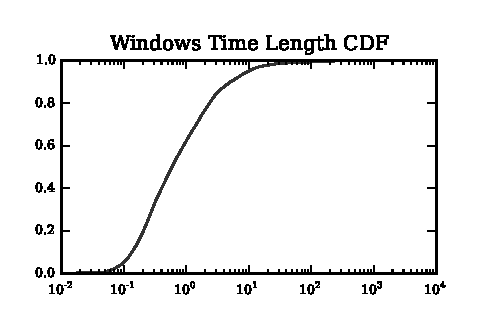
\includegraphics[scale=1]{./figures/window_time_size_histogram.eps}
\caption{Cumulative distribution function for the time length of the windows given in hours. Most windows' lengths are in the interval $[10^{-1}, 10^1]$ hours; about 60\% of windows are 1 hour or less, meaning users receive on average over 100 tweets an hour.}
\label{fig:window_time_size_histogram}
\end{figure}

\subsection{How prevalent are non-explicit responses?}

This section addresses the first research question \ref{rq:similarityPotential} of whether or not text similarity has potential for identifying untagged responses, starting with whether Tagged reactions indeed tend to have higher scores than Non-Tagged ones. 

\begin{table}[!tb]
	\centering
	\fontsize{9pt}{10pt}\selectfont
		\begin{tabular}{l|c|c|c|}
			\cline{2-4}
												& Mean					& Median					& Std. \\ \hline 
			\multicolumn{1}{|l|}{Non-Tagged}	& \nonTaggedScoreMean{}	&	\nonTaggedScoreMedian{}	& \nonTaggedScoreStd{} \\ \hline
			\multicolumn{1}{|l|}{Replies}		& \repliesScoreMean{}	&	\repliesScoreMedian{}	& \repliesScoreStd{} \\ \hline
			\multicolumn{1}{|l|}{Retweets}		& \retweetsScoreMean{}	&	\retweetsScoreMedian{}	& \retweetsScoreStd{} \\ \hline
		\end{tabular}
\caption{Sample mean and standard deviation for the normalized similarity score for the Replies, Retweets, and Non-Tagged sets.}
	\label{tab:sampleDistributionsStatistics}
\end{table}

\begin{figure}[!htbp]
\centering
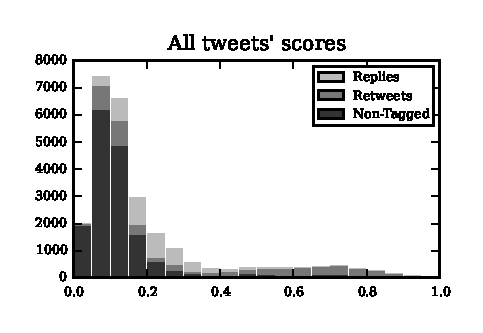
\includegraphics{./figures/all_tfidf_histogram.eps}
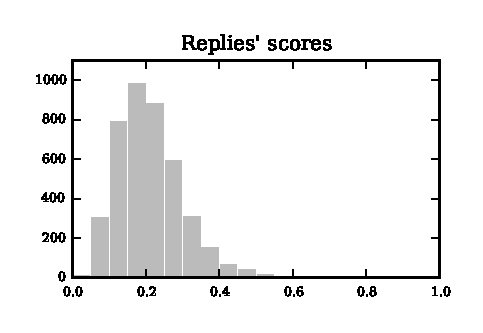
\includegraphics{./figures/replies_tfidf_histogram.eps}
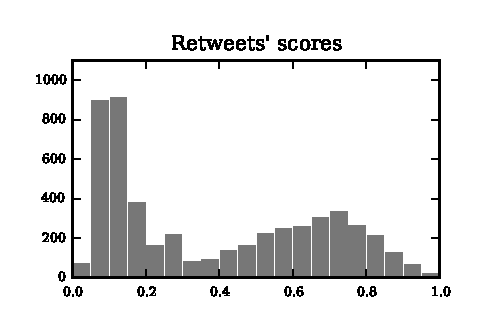
\includegraphics{./figures/retweets_tfidf_histogram.eps}
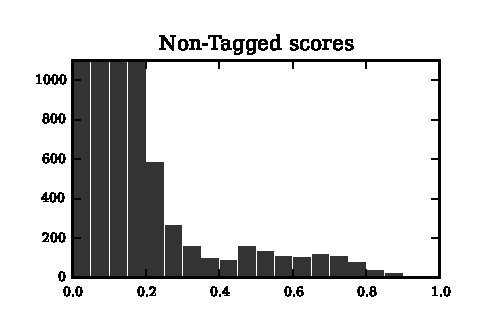
\includegraphics{./figures/not_retweets_replies_tfidf_histogram_cutoff_y.eps}
\caption{Histograms for the normalized similarity scores.  Note that the y-axis for the Non-Tagged subgraph was truncated at 1100 for better visualization of the tail of the distribution and matching other scales.  Retweets have a higher average score than Replies, which in turn are higher than Non-Tagged.  Further, Retweets have a bimodal distribution; high scores are near-duplicates of the tweets they are responding to, but over \lowRetweetCountPct{}\% have a score below \thresholdScore{}, suggesting that people often substantially edit retweets or retweet items not in their feed windows.}
\label{fig:fig_tweets_histograms}
\end{figure}

Mean and median scores are lowest for Non-Tagged and highest for Retweets, as shown in Table \ref{tab:sampleDistributionsStatistics}. This can also be seen in the scores' histogram for each of these sets in Figure \ref{fig:fig_tweets_histograms}. The score behaves as expected when we consider the averages, returning higher values for Replies and Retweets. However, the proximity of the means for the Replies and Non-Tagged and the higher variance of the Non-Tagged makes these two distributions not so well distinguishable based on score alone. The Retweets, on the other hand, present a heavier tail on the distribution. This suggests that the score captures general trends of the Tagged tweets, but is more suitable for Retweets. Considering that the Retweet average is \thresholdScore{} and that it is higher than the Replies mean by more than one standard deviation, \textbf{high scored messages} are defined as messages with $score \geq \thresholdScore{}$.
%% DC 26: It would be pretty straightforward to run something like a chi-square test to argue that the distributions are or are not significantly different (where you talk about "not so well distinguishable")

Although the Non-Tagged set has a lower average, it has a higher variance than replies. This comes from the fact that Non-Tagged tweets have a heavier tail when compared to replies, as seen in Figure \ref{fig:fig_tweets_histograms}. Also, the Non-Tagged high scored tweets are not neglectable when compared with the number of high scored Tagged tweets, as seen in Table \ref{tab:highScoredCounts}: such Non-Tagged tweets would comprise about \highNonTaggedTweetCountPct{}\% of responses, even with a fairly conservative cutoff of \thresholdScore{}. However, high scored messages misses most of the explicit Replies with this cutoff choice.

\begin{table}[!tb]
	\centering
	\fontsize{9pt}{11pt}\selectfont
		\begin{tabular}{l|>{\centering\arraybackslash}m{1.6cm}|>{\centering\arraybackslash}m{1cm}|>{\centering\arraybackslash}m{1.1cm}|}
			\cline{2-4}
			& Non-Tagged & Replies & Retweets \\ \hline
			\multicolumn{1}{|p{2.2cm}|}{\parbox[top][22pt][c]{2.2cm}{High Scored\\($score \geq \thresholdScore{}$)}} & 
			\cellcolor{gray!25} \highNonTaggedTweetCount{} & \highRepliesTweetCount{} & \highRetweetsTweetCount{} \\ \hline
			\multicolumn{1}{|p{2.2cm}|}{Total} & 
			\totalNonTaggedTweetCount{} & \cellcolor{gray!25} \totalReplies{} & \cellcolor{gray!25} \totalRetweets{} \\ \hline
		\end{tabular}
		\caption{Number of high scored messages and the total of messages for the sets Non-Tagged, Replies and Retweets. The highlighted number of high scored Non-Tagged messages is around \highNonTaggedTweetCountPct{}\% of the highlighted total of Tagged messages.}
	\label{tab:highScoredCounts}
\end{table}

Considering the retweet behavior, it would be expected that the normalized similarity score for retweeted messages would be high as long as the original tweet showed up in the windows and the retweet is basically reproducing the message with almost no modifications. 
Surprisingly, this is not what is observed in Figure \ref{fig:fig_tweets_histograms}.  Instead, more than \lowRetweetCountPct{}\% of Retweets have a $score < \thresholdScore{}$.  One possible explanation for this is that people sometimes retweet when they use other parts of the interface, such as other users' profiles or search results, or use social media share buttons attached to tweets on other sites.  Another possibility is that people might frequently edit retweets.

\subsection{Features of Replies, Retweets and Non-Tagged messages}

To help understand the mystery of low-scoring retweets, and more generally to understand what sorts of markers the method is using to identify potential responses, a sample of representative tweets from each category across a range of normalized similarity scores is examined.  
Tables \ref{tab:tweetsScoresRetweets}, \ref{tab:tweetsScoresReplies} and \ref{tab:tweetsScoresNonTagged} (see the Appendix) show both the user's tweet (top in each pair) and the text of the highest-scoring followee's tweet in the window for that tweet (bottom in each pair).

For system tagged Retweets, most of the high scored content has almost the same content as the original message (as expected), as in tweets \#1 and \#2 in the table.  One interesting thing to notice here is that as the tweet length decreases, the normalized similarity score goes down (compare \#6 to \#1). This is related to the fact that the $tf\mhyphen idf$ score is sensitive to the number of matched words between the query and the document.  
Below a threshold of around $0.3$ in this dataset, this effect disappears.  Instead, the text starts to look more like 
two tweets about a common external topic (\#7, \#8, \#9)---despite the fact that the tweet text preserves the ``RT'' retweet marker.  These would be likely candidates for actual retweets that occur outside the window, either farther back in the feed or other parts of the interface than the feed.

When looking at system tagged Replies, high-scoring replies show two main patterns.  In one, they look largely like retweets that were tagged as replies, likely because people pressed the reply button and pasted text from the text they replied to, as in \#11.  In the other, the tweet mentions multiple users who are conducting an ongoing conversation and want all of them to be notified when someone posts something new, as in \#12 and \#13.  It is important to notice that this set of tweets has a maximum score lower than the other sets; scores on the higher end of the distribution could not be found. Also, it appears that @-mentions are the main source of evidence for the normalized similarity scoring even as it goes down, and in fact, replies with low scores still often look like replies despite the low $tf\mhyphen idf$.  This is often (\#16, \#19) but not always (\#18, \#20) indicated by bi-directional @-mentions of the conversational partner.

When looking at Non-Tagged tweets, one of the first things to notice is that high scored tweets usually are retweets that were not captured by the system.  In some cases it is likely users are manually copying the content of the messages and adding retweet markers (\#23, \#24); in others, it is more likely that both users are independently retweeting external content (\#21, \#22).  Users often make small comments together with the original text (\#22, \#23, \#25).  As the normalized similarity score goes down, the messages look less like a retweet, but often still appear to be topically related, sometimes via hashtags (\#28, \#29).  

In general, higher normalized similarity scores seem to capture retweets reasonably well, even though being sensitive to their length, and a particular type of reply that involves conversations.  Non-tagged tweets with high scores are often retweets or quotes with extra comments from the users, although sometimes the retweets may be common retweeting of external content rather than retweets from the window.
%% DC 16: I don't really believe the following argument: #21 and 22 look much more like external stimulus to me.
%One initial concern about using text similarity was that it would be hard to distinguish actual responses from situations where people comment on a common external stimulus.  
%In these data, however, high scores appear to be reliably associated with responses rather than external stimulus.
Further, even the conservative estimate chosen shows that non-explicit responses are quite common---and it is likely that a number of the of the ``middle scoring'' tweets are actual responses.  Distinguishing those from external influences or underlying interest similarity would be an important next problem in building better models of non-explicit response.  

\subsection{Variations in User Responsiveness}

The previous sections demonstrate that it is likely that \highNonTaggedTweetCountPct{}\% or more of Non-Tagged tweets are responses that are not explicitly captured by the system.  This section addresses the other main research question \ref{rq:usersDistribution} of how these losses are distributed among different users in the network.   

These Non-Tagged high-scored messages were authored by \highUserCount{} of the \totalUsers{} users (\highUserCountPct{}\%). This suggests that users generate responses that are missed in a non-uniform way: many users behave as the system expects, using explicit reply and retweet mechanisms, but a significant number respond, at least sometimes, without using those mechanisms. 
Figure \ref{fig:users_reponse_histograms} shows histograms for example users that have most or all of their responses untagged by Twitter even though they present a high $score$.  Note that these users span a range of activity levels, meaning that they are not just newbies that do not know how to use the interface.

\begin{figure}[!tb]
\centering
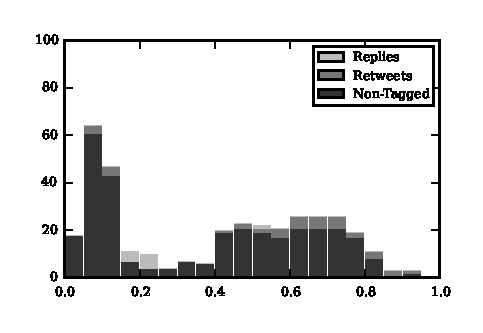
\includegraphics[scale=0.9]{./figures/213501392_histogram.eps}
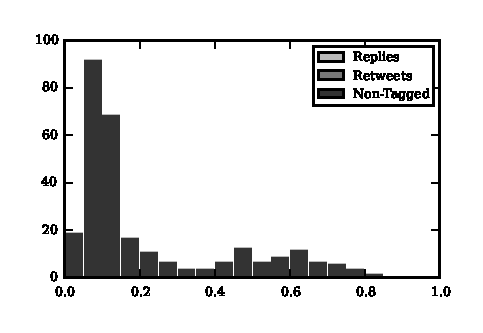
\includegraphics[scale=0.9]{./figures/808181892_histogram.eps}
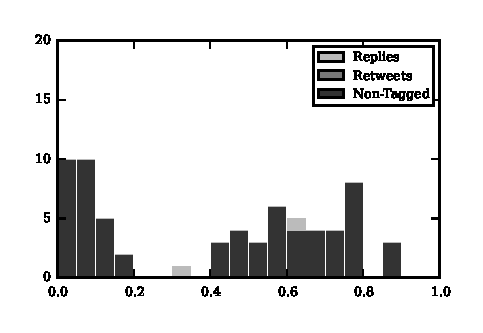
\includegraphics[scale=0.9]{./figures/87339782_histogram.eps}
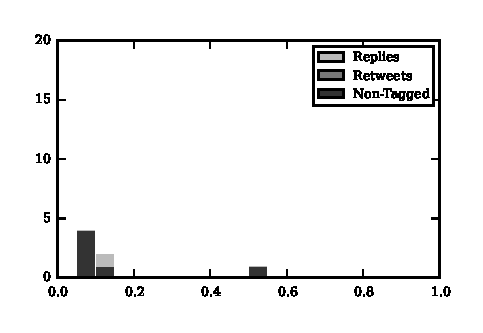
\includegraphics[scale=0.9]{./figures/196322186_histogram.eps}
\caption{Score histograms for sample users who present a significant amount of high scored Non-Tagged content relative to their total amount of messages, which indicates that most of their reactions are not being properly tagged by Twitter.}
\label{fig:users_reponse_histograms}
\end{figure}


In order to better understand the behavior distribution among all users, Figure \ref{fig:2d_histogram} shows a 2d-histogram for the points $(p_i^T, p_i^N)$, where each of these points is the percentage of the Tagged messages $p_i^T$ and the percentage of the high scored Non-Tagged messages $p_i^N$.  Each of these points is evaluated for a user $u_i$ in relation to the total number of messages the user authored.
The high scored Non-Tagged percentage $p_i^N$ is the proportion of this user behavior that were likely to be reactions while the percentage $p_i^T$ is the proportion of reactions actually captured.


The \usersScoreZero{} users that never have messages that scored higher than $\thresholdScore{}$ nor used explicit system reply mechanisms are concentrated at the origin of the histogram.
Users that lay on the $x$-axis only react through explicit reaction mechanisms the system offers, therefore have all their reaction Tagged. Similarly, users on the $y$-axis never use explicit reaction mechanisms, although they present high scored Non-Tagged content. Users above the dashed line have more high scored Non-Tagged content than Tagged content. It is possible to say that users that lay above the dashed line are more likely to produce content that can be missed by Twitter's tagging system, and they account for \usersAboveLine{} users, about $\usersAboveLinePct{}\%$ of the dataset. 

\begin{figure}[!tb]
\centering
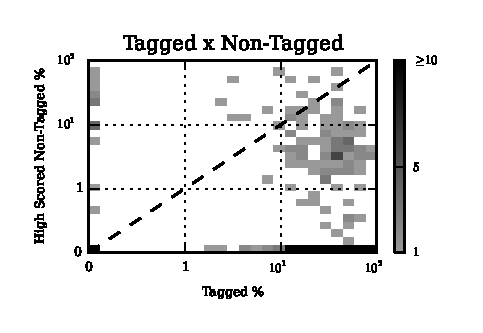
\includegraphics[scale=1.2]{./figures/user_alltagged_highnontagged_2dhist_0375.eps}
\caption{2D histogram of the percentage of Tagged and high-scored Non-Tagged messages for all users. The scale is linear in the interval $[0,1]$ and logarithmic on the interval $(1,100]$; the dashed line represents an equal percentage of Tagged and Non-Tagged tweets. 
Many users are non-responsive (the point at the origin) or use the explicit response mechanisms consistently (points hugging the x-axis with a 0 value for high scored Non-Tagged \%).  However, a significant number never use the explicit response mechanisms (points hugging the y-axis with a 0 value for Tagged \%), use them only occasionally (points above the dashed line), or occasionally forget to use them (points below the dashed line).}
\label{fig:2d_histogram}
\end{figure}


\begin{figure}[!tb]
\centering
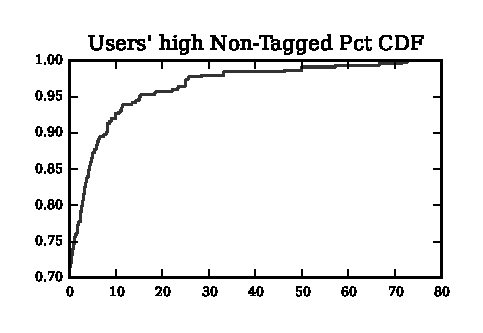
\includegraphics[scale=1]{./figures/users_high_nontagged_pct_cdf.eps}
\caption{Cumulative distribution of the users for the percentage of high scored Non-Tagged messages. \usersZeroHighScoredPct{}\% of the users have no high scored Non-Tagged messages, while \usersMoreThanTenPctPct{}\% of the users had at least 10\% of their messages high scored and Non-Tagged.}
\label{fig:cumulative_user}
\end{figure}


When considering the cumulative distribution of the users according to the percentage of high scored Non-Tagged messages $p_i^N$, shown in Figure \ref{fig:cumulative_user}, we identify more than \usersMoreThanTenPctPct{}\% of the users with at least 10\% of their messages being high scored and missed by Twitter's tagging system. 

These results indicate that methods that rely on explicit indicators of response likely miss or seriously under-represent the behavior of a sizable proportion of the Twitter population.


\chapter{Averaging Gone Wrong: Using Time-Aware Analyses to Better Understand Behavior}
\label{ch:cohorts}

Understanding the evolution of users in a social network is essential for a variety of tasks: monitoring community health, predicting individual user trajectories, and supporting effective recommendations, among others.  Many works aim at explaining these temporal aspects of evolution. Some adopt a point of view of the whole network and try to understand general patterns of behavior \cite{Zhu2014, Kooti2010}, while others adopt a user-centric point of view and try to model \cite{Correa2010, Priedhorsky2007, Panciera2009, Welser2011} or predict \cite{Danescu-niculescu-mizil2013} individuals' behavior.

These approaches often combine all available data into aggregate analyses of the whole community over its entire history.  This can be a natural response to limitations in the amount of available data:  datasets may capture a small part of the community's history \cite{Artzi2012}; timestamps may not be available \cite{Priedhorsky2007, Pujol2010}; snapshots may provide limited views of the community \cite{Cosley2010}; or the community itself may be small \cite{Lewis2008}.  Aggregate time-based analyses are also a natural first way to address questions of community evolution.

However, we argue that many of these aggregated views are misleading. The conditions under which users join the community may vary greatly over time in ways that might impact their behavior \cite{Miller2015}.  Among other things, popularity, purpose, features, interface, and algorithms can change: Wikipedia circa 2005 and circa 2015 are very different, as are Facebook of 2005 and 2015.  Analyses---including some of our own past work---that fail to account for this change may miss important details of what is really going on.

We support this argument through an analysis of user effort in Reddit, one of the most popular and long-running online communities, based on a very large, recently released dataset of posting behavior.  We address a number of questions commonly raised about users' effort in online communities: how active are users, how hard do they work, and what kinds of things do they do?  In each case, we compare aggregate analyses of posting behavior to ones that treat users in Reddit as yearly cohorts, and views that focus on calendar time versus user-referential views that normalize behavior based on the date of a user's first visible activity.  We also look at differences within yearly cohorts, focusing on how behavior differs between shorter and longer-lived users within each cohort \cite{Barbosa2016}.

We find that these accountings for time reveal insights about Reddit beyond what commonly performed aggregate analyses can provide.  Users who join Reddit earlier post more and longer comments than those who join later, while users who survive longer start out both more active and more likely to comment than submit versus users who leave Reddit early; none of these findings are obvious from aggregate views of user behavior.  

Further, we find that aggregate analysis can be downright misleading.  For instance, although average comment length decreases over time in an aggregate view, the comment length for surviving users increases over time in every cohort.  Likewise, an aggregate analysis suggests that longer-lived users post more over time; this is not the case.  Instead, users come into Reddit as active as they will ever be (akin to Panciera et al.'s finding that Wikipedians are ``born, not made'' \cite{Panciera2009}), and the rise in average activity for surviving users over time is driven by lower-activity users leaving early.

We see the second part of this thesis as both making specific contributions to understanding behavior in Reddit and a more general contribution around the importance of considering change over time in analyzing online communities. 

\section{Time matters} 

\subsection{Why accounting for time is important}

Communities grow and, with time, die. For any community, its users play a role in its evolution, but they are also simultaneously affected by the evolution of the community. Untangling this interplay can help make sense of patterns of activity in a community.

One useful way to understand the evolution of a community and its users is through time, as it provides a linear account of the growth (or decay) of overall activity, types of content, and social norms and structure.  One aspect of time often considered is the tenure of a user in the community, as in studies around modeling users' preferences \cite{McAuley2013} or analyzing the evolution of their language \cite{Danescu-niculescu-mizil2013}.  These analyses uncover insights about the lifecycle of a user in a community: users' preferences and behavior change with their age in a community \cite{Panciera2010}, while their early experiences and activity shape future outcomes predictably \cite{Tan2015,Yang2009,Panciera2009, Miller2015}. 

However, much past work on online communities ignores the time at which a user joins the community and analyzes all users together.
This might be a mistake: communities may grow denser or sparser with time \cite{Leskovec2005}, develop new norms \cite{Kooti2010}, and enact policies and rules guiding people's behavior \cite{Butler2008}.
These changes mean that people experience different versions of a community at different times, which can, in turn, affect their observed behavior. This interaction with the state of a community can confound conclusions about people's behavior, because the differences one observes may simply due to changes in the community, rather than any significant change in the outcome variable of interest or the user population.  


\subsection{Cohorts are analytically useful}

A common method to control for such confounds is cohort analysis, widely used in fields such as sociology \cite{Mason2012,Glenn2005}, economics \cite{Attanasio1993,Beldona2005}, and medicine \cite{Howartz1996,Davis2010}. A cohort is defined as a group of people who share a common characteristic, generally with respect to time. For example, people born in the same year, or those who joined a school at the same time, or got exposed to an intervention at similar times can be considered as cohorts.  People in a cohort are assumed to be exposed to the same state of the world and thus are more comparable to each other than to people in other cohorts. 

For example, sociological studies often use students who join a school in the same year to understand the effect of interventions \cite{Goyette2008,Alexander2012}, and condition on the year in which people were born to understand people's  behavior, such as variations in financial decision-making \cite{Attanasio1993} or opinions on issues \cite{Firebaugh1988,Jennings1996}. Similarly, medical studies interpret effects of drugs using cohorts of people within the same age group or amount of exposure to correlated conditions \cite{Howartz1996,Davis2010}.  

Recent work shows that cohorts' importance transfers to online communities as well. Just as people's behavior varies according to their biological age, their experience in an online community may vary with their age in the community and their year of joining. In Wikipedia, we find substantial differences in the activities of cohorts of users who joined earlier versus those who joined later \cite{Welser2011}. Similarly, on review websites, users who join later tend to adopt different phrases than the older users who had joined earlier \cite{Danescu-niculescu-mizil2013}.

\subsection{What might cause these differences?}

These differences in activity between cohorts may be due to a number of reasons.  One plausible explanation is selection effects: people who are enthusiastic about a community or its goals are more likely to self-select as early members of a community, while others may be more likely to join later \cite{Li2008}.  In this case, users who join earlier might be expected to be more active, committed users than those who join later. 

Another possible explanation is that community norms may change over time.  In many cases, it is a bottom-up process. Kooti et al. showed that social conventions can define the evolution of a community and the early adopters play a major role in designing these conventions, consciously or not \cite{Kooti2010}. Examples include adoption of `RT', a retweeting norm by Twitter users and the subsequent introduction of the Retweet button on Twitter \cite{Kooti2010}; change in language use between new and old users on review websites \cite{Danescu-niculescu-mizil2013}; and assumptions of clear roles and responsibilities on Wikipedia \cite{Kittur2007a}. In other cases, it may be directed by the community managers. For instance, the makers of Digg unilaterally changed the nature of the community by introducing a new version of the website, leading to a sudden change in norms and behavior in the community \cite{Ingram2014,Lardinois2014}. 

The growth of a community may also affect people's behavior. Successful communities often grow very rapidly, which can be both good and bad for users' experience. On one hand, growth would imply availability of a larger chunk of content to choose from. On the other, it might be harder to connect to others and get responses in a bigger community. A community may also need to adopt new rules and policies to manage growth and newcomers, as in the evolution of Wikipedia \cite{Choi2010,Bryant2005}. In those cases, the experience of later cohorts of users may be vastly different from the initial ones who joined before formal rules were in place. 

Finally, patterns of use may change because the overall population of Internet users is still changing.  As more and different people come online, their influx may lead to changes in activity patterns and communities (as with the yearly entry of college freshmen, and eventually all of AOL, gaining access to Usenet).  The gradual penetration of technology also has age-related effects:  people who did not grow up in a technological environment differ in their social media and search usage compared to younger generations\cite{Correa2010,Beldona2005}. 

\subsection{Is Reddit getting ``worse'' over time?}
All of the above reasons suggest that users from different cohorts are likely to be different, which has also been demonstrated in online and offline communities \cite{Ryder1965,Danescu-niculescu-mizil2013,Prensky2001,Correa2010}.  Further, they suggest a general hypothesis that communities ``get worse'' over time because newer users are likely to be less committed and knowledgeable about the community. 

To address this hypothesis, we analyze both aggregate and cohort-based measures of user quality that are often raised about online communities: how active are users \cite{Scellato2011,Hughes2009,Java2007,Levy1984}, how much do they contribute \cite{Scellato2011,Gruhl2004,Guo2009}, and what kinds of work do they engage in \cite{Welser2011,Choi2010,Panciera2009}?  

We do this in the context of Reddit, a community that has been studied by many researchers \cite{Gilbert2013,Stoddard2015,Bergstrom2011,Tan2015}. We begin with a brief overview of both Reddit and the dataset that we use in this work, focusing on aspects that directly impact our analyses\footnote{There is more to say about Reddit itself (see \cite{AboutReddit}).}.

\section{Data: Reddit as a community}

%% DC 14: Moving this to the end of prev work to give a little more context and beef; things felt redundant between that and this and it feels better there.

\subsection{What is Reddit, briefly}

%% Sam 11: Improving the caption
\begin{figure}[!tb]
\centering
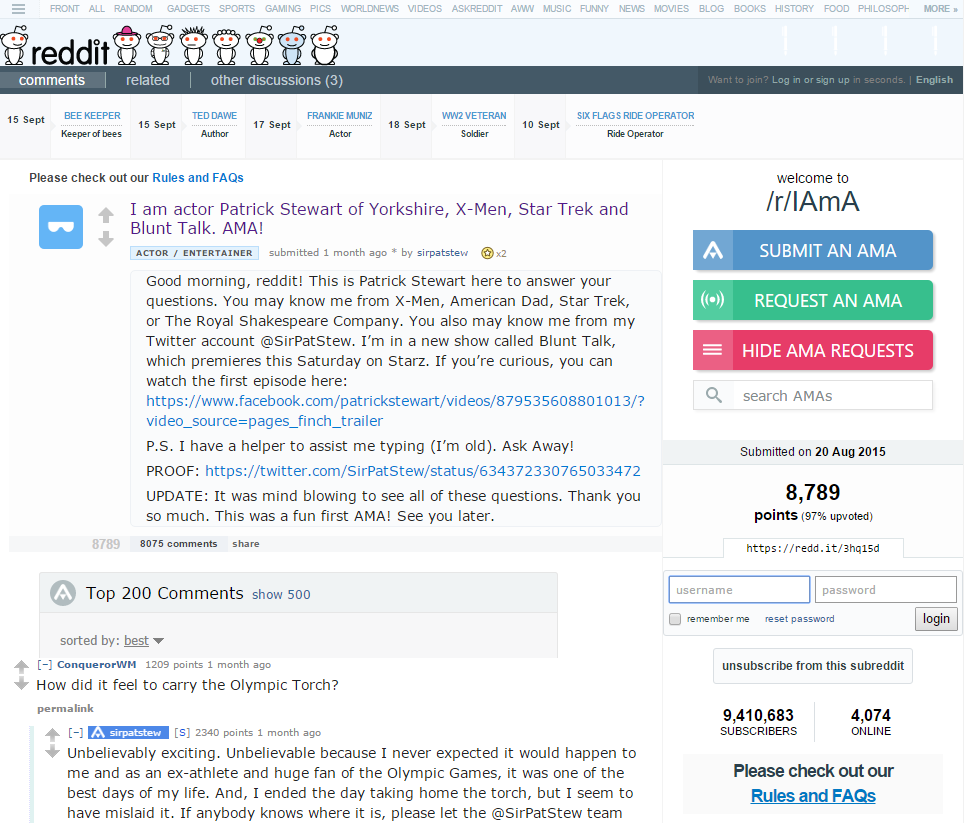
\includegraphics[width=0.45\textwidth,natwidth=964,natheight=823]{./images/reddit.png}
\caption{Reddit interface when visualizing a submission. This is Patrick Stewart's ``AmA'' (ask me anything) in ``IAmA'' (I am a), a submission where he answers users' questions in the comments. We can see the most upvoted comment and Patrick's answer right below.}
\label{fig:reddit}
\end{figure}

Reddit is one of the largest sharing and discussion communities on the Web.  According to Alexa, as of late 2015 Reddit is in the top 15 sites in the U.S. and the top 35 in the world in terms of monthly unique visitors.  It consists of a large number of subreddits (853,000 as of June 21st, 2015\footnote{\cite{RedditStatistics} provides more statistics about Reddit.}), each of which focuses on a particular purpose.  Many subreddits are primarily about sharing web content from other sites: in ``Pics'', ``News'', ``Funny'', ``Gaming'', and many other communities, users (``Redditors'') make ``submissions'' of links posted at other sites that they think are interesting.  In other subreddits, Redditors primarily write text-based ``self-posts'': ``AskReddit'', ``IAmA'', and ``ShowerThoughts'' are places where people can ask questions and share stories of their own lives.  Generically, we will refer to submissions and text posts as ``submissions''.  

Each submission can be imagined as the root of a threaded comment tree, in which Redditors can comment on submissions or each other's comments.  Redditors can also vote on both submissions and comments; these votes affect the order in which submissions and comments are displayed and also form the basis of ``karma'', a reputation system that tracks how often people upvote a given Redditor's comments and submissions. We can observe these elements in Figure~\ref{fig:reddit}. 
%% DC 14: Not so relevant here, so cutting. Redditors can also create subreddits and volunteer to moderate them.

We choose Reddit as our target community for a number of reasons.  It has existed since 2005, meaning that there has been ample time for the community to evolve and for differences in user cohorts to appear.  Second, it is one of the most popular online communities, allowing different types of contributions---comments and original submissions---across many different subreddits.  Third, a number of Reddit users believe that it is, in fact, getting worse over time\cite{RedditWorse1,RedditWorse2,RedditWorse3,RedditWorse4,RedditWorse5,RedditWorse6}. Finally, Reddit data are publicly available through an API.

\subsection{The dataset}

\begin{figure*}[!tb]
\centering
\subimage[width=0.48, scale=0.40]{./images/cumulative_users_subreddits.eps}
\subimage[width=0.48, scale=0.40]{./images/active_users_subreddits.eps}
\caption{Figure (a) shows the cumulative growth of Reddit for users and subreddits. Figure (b) shows the number of active users and subreddits in Reddit over time. An active user or subreddit is one that had at least one post (comment or submission) in the time bin we used---here, discretized by month.}
\label{fig:cumulative}
\end{figure*}

Redditor \textit{Stuck\_In\_The\_Matrix} used Reddit's API to compile a dataset of almost every publicly available comment\cite{RedditDataset1} from October 2007 until May 2015.  The dataset is composed of 1.65 billion comments, although due to API call failures, about 350,000 comments are unavailable.  He also compiled a submissions dataset for the period of October 2007 until December 2014 (made available for us upon request) containing a total of 114 million submissions.  These datasets contain the JSON data objects returned by Reddit's API for comments and submissions\footnote{A full description of the JSON objects is available at \cite{RedditAPI}.}; for our purposes, the main items of interest were the UTC creation date, the username, the subreddit, and for comments, the comment text.

\looseness=-1
We focus on submissions and comments in the dataset because they have timestamps and can be tied to specific users and subreddits, allowing us to perform time-based analyses.   In some analyses, we look only at comments; in some, we combine comments and submissions, calling them \textbf{``posts''}.  We would also like to have looked at voting behavior as a measure of user activity\footnote{This would also give us more insight than usual into lurkers' behavior; we'll return to this in the discussion.}, but individual votes with timestamps and usernames are not available through the API, only the aggregate number of votes that posts receive.

\subsection{Preprocessing the dataset}

\looseness=-1
To analyze the data, we used Google BigQuery\cite{BigQuery}, a big data processing tool.
Redditor \textit{fhoffa} imported the comments into BigQuery and made them publicly available\cite{RedditDataset2}.  We uploaded the submission data ourselves using Google's SDK.

For the analysis in the work, we did light preprocessing to filter out posts by deleted users, posts with no creation time, and posts by authors with bot-like names\footnote{Ending with ``\_bot'' or ``Bot''; or containing ``transcriber'' or ``automoderator''.}.
%% DC 14: Would like to at least informally be able to address the critique that this doesn't capture all bot activity and excludes some legit users by giving a feel for the scope of the problem.

We also considered only comment data from October 2007 until December 2014 in order to have a matching period for comments and submissions. After this process, we had a total of 1.17 billion comments and 114 million submissions.

\subsection{An overview of the dataset}

Here we present an overview of the dataset that shows Reddit's overall growth.  Figure~\ref{fig:cumulative}a presents the cumulative number of user accounts and subreddits created as of the last day of every month. After an initial extremely rapid expansion from 2008--2009, the number of users and subreddits have grown exponentially.  As of the end of 2014, about 16.2 million distinct users and 327 thousand subreddits made/received at least one post based on our data.

%% Sam 8: There was a problem in my query for the active users, I was counting less than I should. I replaced the text with the right numbers, but they might not be considered ``and order of magnitude less'' now, more like 5x less
However, as with many other online sites, most users \cite{Scellato2011,Hughes2009,Java2007} and communities \cite{Arguello2006} do not stay active. We define as an ``\textbf{active user}'' one that made at least one post in the month in question. Similarly, an ``\textbf{active subreddit}'' is one that received at least one post in the month. In December 2014, about 2.7 million users and 66 thousand subreddits were active, both around a fifth of the cumulative numbers. Figure~\ref{fig:cumulative}b shows the monthly number of active users and subreddits.

Our interest in this work is not so much whether users survive as it is about the behavior of active users.  Thus, 
in general our analysis will look only at active users and subreddits in each month; those that are temporarily or permanently gone from Reddit are not included.  

\subsection{Identifying cohorts}

\begin{figure*}[!tb]
\centering
\subimage[width=0.48, scale=0.40]{./images/avr_posts_per_user_over_time_total.eps}
\subimage[width=0.48, scale=0.40]{./images/avr_posts_per_user_user_ref_total.eps}
\caption{In Figure (a), monthly average posts per active user over clock time. In Figure (b), monthly average posts per active users in the user-time referential, i.e., message creation time is measured relative to the user's first post.  Each tick in the x-axis is one year.  In both figures (and all later figures), we consider only active users during each month; users that are either temporarily or permanently away from Reddit are not included.}
\label{fig:overall_posts}
\end{figure*}

We define the ``\textbf{user's creation time}'' as the time of the first post made by that user.  Throughout this work, we will use the notion of user cohorts, which will consist of users created in the same calendar year.

In many cases, we will look at the evolution of these cohorts. Since users can be created at any time during their cohort year, and our dataset ends in 2014, 
we are likely to have a variation on the data available for each user of up to one year, even though they are in the same cohort.  To deal with this, some of our cohorted analyses will consider only the overlapping time window for which we collect data for all users in a cohort.   This means that we are normally not going to include the 2014 cohort in our analyses.

Our data starts in October 2007, but Reddit existed before that. That means that, not only do we have incomplete data for the 2007 year (which compromises this cohort), but there might also be users and subreddits that show up in 2007 that were actually created in the previous years. Since we can not control for these, we will also omit 2007 cohort. We will, however, include 2007 in the overall analyses over time (the non cohorted ones) for two reasons: first, it does not have any direct impact on the results; second, we often compare the cohorted approach with a naive approach based on aggregation, and we would not expect a naive approach to do such filtering. 


\section{Average posts per user}
One common way to represent user activity in online communities is quantity: the number of posts people make over time. Approaches that consider the total number of posts per user in a particular dataset \cite{Gruhl2004} and that analyze the variation of the number of posts per user over time \cite{Guo2009} have been applied to online social networks.  In this section, we use this measure to address our first research question (\ResearchQuestion\label{rq:activityChange}): how does the amount of users' activity change over time?

As we will see, both visualizing behavior relative to a user's creation time and using cohorts provide additional insight into posting activity in Reddit compared to a straightforward aggregate analysis based on calendar time.

\subsection{Calendar versus user-relative time}

Figure~\ref{fig:overall_posts}a shows that aggregate analysis, presenting the average number of posts per month by active users in that month.  Taken at face value, this 
suggests that over the first few years of Reddit, users became more active in posting, with per-user activity remaining more or less steady since mid-2011.

\looseness=-1

%% Sam 8: Reorganized the next 3 paragraphs, added information about throw away accounts
This average view hides several important aspects of users' activity dynamics. Previous work has looked into behavior relative to the user creation time. It has been shown that edge creation time in a social network relative to the user creation follows an exponential distribution \cite{Tomkins2008}. User lifetime, however, does not follow a exponential distribution and some types of user content generation follow a stretched exponential distribution \cite{Guo2009}. Throw-away accounts are one example of very short-lived users in Reddit \cite{Bergstrom2011}, for example. 

To address these characteristics, Figure~\ref{fig:overall_posts}b shows a view that emphasizes the trajectory over a user's lifespan rather than the community's.  To do this, we scale the x-axis not by clock time, as in Figure~\ref{fig:overall_posts}a, but by time since the user's first post: ``1'' on the x-axis refers to one year since the user's account first post, and so on. We call this the \textbf{time in the user referential}. One caution about interpreting graphs with time in the user referential is that the amount of data available rapidly decreases over time as users leave the community, meaning that values toward the right side of an individual data series are more subject to individual variation.  

%% Sam 11: Treating the misinterpretation as a hypothesis
%% Sam 12: The point of highlighting this as hypothesis is to point out at the end all the possible mistakes.
The evidence at this point supports the tempting hypothesis that the longer a user survives, the more posts they make (\Hypothesis\label{hyp:survivingMorePosts}).  This hypothesis, however, is incorrect; we will present a more nuanced description of what is happening informed by cohort-based analyses.

\subsection{New cohorts do not catch up}

\begin{figure*}[!tb]
\centering
\subimage[width=0.48, scale=0.42]{./images/avr_posts_per_user_over_time_cohorts.eps}
\subimage[width=0.48, scale=0.42]{./images/avr_posts_per_user_cohorts.eps}
\caption{Figure (a) shows the average number of posts per active user over clock time and Figure (b) per active user in the user-time referential, both segmented by users' cohorts. The user cohort is defined by the year of the user's creation time.  For comparison, the black line in Figure (a) represents the overall average.}
\label{fig:avr_posts_per_user_over_time_cohorts}
\end{figure*}

%% Sam 12: Adding the first research question here because we start cohorting here, and that is the main strategy of the paper.
%% DC 14: Didn't work as-is since it's not parallel with the others, and was referred to in the more general way in the discussion/conclusion section, so added a general version earlier and changed the label for this one.
Figure~\ref{fig:overall_posts}b suggests that older users are more active than newer ones, raising the question of whether new users
eventually follow in older users' footsteps (\SubResearchQuestion\label{srq:newFollowOld}).  

Analyzing users' behavior by cohort is a reasonable way to address this question, and Figure~\ref{fig:avr_posts_per_user_over_time_cohorts}a shows a first attempt at this analysis.  We can already observe a significant cohort effect: users from later cohorts appear to level off at significantly lower posting averages than users from earlier ones.  It suggests that newer users likely will never be as active as older ones on average.  It also shows that surviving users are significantly more active than the overall average (the black line in the figure) would suggest.

However, Figure~\ref{fig:avr_posts_per_user_over_time_cohorts}a also has an awkward anomaly: a rapid rise in the average number of posts during each cohort's first calendar year, especially in December. Combining cohort segmentation with user-referential analysis, as in Figure~\ref{fig:avr_posts_per_user_over_time_cohorts}b, helps smooth out this anomaly and aligns cohorts with each other.  Doing this alignment makes clear that differences between earlier and later cohorts are apparent early on.

\subsection{Does tenure predict activity, or vice versa?}

\begin{figure*}[!tb]
\centering
\subimage[width=0.31, scale=0.29]{./images/avr_posts_per_user_for_surviving_year_for_2010.eps}{2010 cohort}
\subimage[width=0.31, scale=0.29]{./images/avr_posts_per_user_for_surviving_year_for_2011.eps}{2011 cohort}
\subimage[width=0.31, scale=0.29]{./images/avr_posts_per_user_for_surviving_year_for_2012.eps}{2012 cohort}
\caption{Each Figure corresponds to one cohort, from 2010 to 2012, left to right. The users for each cohort are further divided in groups based on how long they survived: users that survived up to 1 year are labeled 0, from 1 to 2 years are labeled 1, and so on.  For all cohorts, longer-tenured users started at higher activity levels than shorter-tenured ones.}
\label{fig:avr_posts_per_user_for_surviving_year}
\end{figure*}

%% Sam 11: Accommodating the hypothesis, adding the second ``correct'' hypothesis
\looseness=-1
These graphs still support our initial hypothesis \ref{hyp:survivingMorePosts} 
%the tempting conclusion that users become more active the longer they exist in Reddit, 
and they do not explain the rapid increase in posting activity in the first few months.  An alternative hypothesis, inspired by the ``Wikipedians are Born, not Made'' paper \cite{Panciera2009}, is that individual users come in with different posting propensities, and the rise over time is not that individual users become more active but that low-activity users leave the system (\Hypothesis\label{hyp:lowActivityLeave}).  To examine this, we further segment each cohort by the number of years they were active in the system, as defined by the difference between their first and last post times.
 
Figure~\ref{fig:avr_posts_per_user_for_surviving_year} shows this analysis for the 2010, 2011 and 2012 cohorts\footnote{We only show these figures for the sake of saving space, but the same trends are observed in the other cohorts.}.  Across all cohorts and yearly survival sub-cohorts, users who leave earlier come in with a lower initial posting rate.  Thus, the rise in average posts per active user is driven by the fact that users who have high posting averages throughout their lifespan are the ones who are more likely to survive.  As the less active users leave the system, the average per active user increases.  In other words, the correct interpretation of Figure~\ref{fig:overall_posts}b is not \ref{hyp:survivingMorePosts}: longer-lived users don't post more as they age.  Instead, users who post more---right from the beginning---live longer, supporting (\ref{hyp:lowActivityLeave}). 

Combining Figure~\ref{fig:avr_posts_per_user_for_surviving_year}'s insight that the main reason why these curves increase is because the low posting users are dying sooner with the earlier observation that the stable activity level is lower for newer cohorts suggests that low-activity users from later cohorts tend to survive longer than those from earlier cohorts.  That is, people joining later in the community's life are less likely to be either committed users or leave than those from earlier on: they are more likely to be ``casual'' users that stick around.

\vspace{7pt} 
\section{Comment length}

\begin{figure*}[!tb]
\centering
\subimage[width=0.48, scale=0.42]{./images/avr_comment_size_over_time_cohorts.eps}
\subimage[width=0.48, scale=0.42]{./images/avr_comment_size_cohorts.eps}
\subimage[width=0.31, scale=0.29]{./images/avr_comment_length_for_surviving_year_for_2010.eps}{2010 cohort}
\subimage[width=0.31, scale=0.29]{./images/avr_comment_length_for_surviving_year_for_2011.eps}{2011 cohort}
\subimage[width=0.31, scale=0.29]{./images/avr_comment_length_for_surviving_year_for_2012.eps}{2012 cohort}
\caption{Figure (a) shows the average comment length over clock time and Figure (b) from the user-referential time. Both figures show the cohorted trends.  The overall average length per comment decreases over time, although for any individual cohort, it increases after a sharp initial drop. Figures (c), (d) and (e), similar to Figure~\ref{fig:avr_posts_per_user_for_surviving_year}, show the monthly average comment length for active users in the cohorts of 2010, 2011 and 2012, segmented by the number of years that the user survived in the network.  Opposite the analysis for average posts, which showed that low-activity users were the first to leave Reddit, here, people who start out as longer commenters are \textit{more} likely to leave.}
\label{fig:comment_length}
\end{figure*}

Activity as measured by the average number of posts per user is one proxy for user effort.  Comment length can also be considered as a proxy for user effort in the network.  Users that type more put more of their time in the network, contribute with more content, and might create stronger ties with the community. Thus, we put forward the following question (\ResearchQuestion\label{rq:commentLengthOverTime}): how does comment length change in the community over time, both overall and by cohort?

\subsection{Comment length drops over time}

%% Sam 11: Adding hypothesis tags. Later on to mention all the possible misleading hypothesis that we can come up with not considering cohorts and time
%% Sam 12: The point of highlighting this as hypothesis is to point out at the end all the possible mistakes.
%% DC 14: Fair enough, but will want to refer to them a little more throughout the text as needed.  In particular, H4 is maybe not a mistake, in the sense that a whole bunch of people coming in and acting differenly might be an instance of that behavior-defining-norms idea from previous work.
Figure~\ref{fig:comment_length}a shows the overall comment length in Reddit over time (the darker line) and the overall length per cohort. 
Based on the downwards tendency of the overall comment length in Figure~\ref{fig:comment_length}a, one might hypothesize that users' commitment to the network is decreasing over time (\Hypothesis\label{hyp:decreasingCommitment}), or that there is some community-wide norm toward shorter commenting (\Hypothesis\label{hyp:communityNorm}). 

However, this might not be the best way to interpret this information. Figure~\ref{fig:comment_length}b shows the comment length per cohort in the user referential time. An important observation here is that younger users start from a lower baseline comment length than older ones. Considering the fact that Reddit has experienced exponential growth, the overall average for Figures \ref{fig:comment_length}a and \ref{fig:comment_length}b is heavily influenced by the ever-growing younger generations, who are more numerous than older survivors and who post shorter comments. 

\subsection{Simpson's Paradox: the length also rises}

Let us go back to Figure~\ref{fig:comment_length}a, which shows the overall average comment length on Reddit over time. We see a clear trend towards declining length of comments in the overall line (the black line that averages across all users). This could be a warning sign for Reddit community managers, assuming longer comments are associated with more involved users and healthier discussions. A data analyst looking at these numbers might think about ways to promote longer comments on Reddit. 

However, Figure~\ref{fig:comment_length}b shows that average comment length increases over time for every cohort. While later cohorts start at smaller comment length, after an initial drop, on average all cohorts write longer comments over time.  This is puzzling: when each of the cohorts exhibits a steady increase in their average comment length, how can the overall mean comment length decrease?  This anomaly is an instance of the Simpson's paradox \cite{simpson1951}, and occurs because we fail to properly condition on different cohorts when computing mean comment length. 

\begin{table}[!tb]
\centering
\tabcolsep=0.07cm
\singlespacing
\fontsize{9pt}{10.5pt}\selectfont
\begin{tabular}{|c|c|c|c|c|c|c|c|c|c|}
\cline{2-9}
\multicolumn{1}{c|}{} & \multicolumn{8}{c|}{Cohorts} \\ \hline
Year & 2007 & 2008 & 2009 & 2010 & 2011 & 2012 & 2013 & 2014 & Overall\\ \hline
2007 & 220 & - & - & - & - & - & - & - & 220 \\ \hline
2008 & 208 & 198 & - & - & - & - & - & - & 204 \\ \hline
2009 & 224 & 204 & 201 & - & - & - & - & - & 208 \\ \hline
2010 & 223 & 204 & 189 & 184 & - & - & - & - & 193 \\ \hline
2011 & 233 & 211 & 199 & 184 & 167 & - & - & - & 182 \\ \hline
2012 & 241 & 221 & 212 & 197 & 173 & 167 & - & - & 178 \\ \hline
2013 & 244 & 225 & 214 & 199 & 177 & 167 & 164 & - & 174 \\ \hline
2014 & 246 & 229 & 217 & 204 & 183 & 172 & 165 & 176 & 176 \\ \hline
\end{tabular}
\caption{Evolution of the average throughout the years for each cohort. Each column here is one cohort and each line is one year in time. Cohorts start generating data in their cohort year, therefore the upper diagonal is blank. On the right column we see the overall average for all users.}
\label{tab:simpson}
\end{table}

Table~\ref{tab:simpson} provides some clues to what might be going on. When we move down the rows, we observe an increasing tendency in each cohort column. It means that the average comment length increases for these users. However, when we move right through the columns, people in later cohorts tend to write less per comment. If we were to average each row, we would still get an overall increasing comment length per year, but that is not what we see in the overall column. What happens here is that the latter cohorts have many more users than earlier ones. Since their numbers increase year by year, we have a much larger contribution from them towards comments, compared to users of earlier cohorts. This uneven contribution leads to the paradox we observed in Figure~\ref{fig:comment_length}a. 

Without the decision to condition on cohorts, one would have gathered an entirely wrong conclusion. People are not writing less as they survive, contra (\ref{hyp:decreasingCommitment}).  Rather, those who tend to write less are joining the community in much larger numbers.  Why later users write less is an open question we speculate about later in the discussion and future work section.
%% DC 14: Didn't feel so convinced by the first half, and the second half is redundant with my rewording above
% Knowing this, one may focus on better onboarding processes for newcomers, or try to learn why users in later cohorts tend to write smaller comments on average.  

\begin{figure*}[!tb]
\centering
\subimage[width=0.48, scale=0.42]{./images/comments_per_submissions_over_time_cohorts.eps}
\subimage[width=0.48, scale=0.42]{./images/comments_per_submissions_cohorts.eps}
\subimage[width=0.35, scale=0.30]{./images/comments_per_submissions_for_surviving_year_for_2008.eps}{2008 cohort}
\subimage[width=0.35, scale=0.30]{./images/comments_per_submissions_for_surviving_year_for_2009.eps}{2009 cohort}
\subimage[width=0.35, scale=0.30]{./images/comments_per_submissions_for_surviving_year_for_2010.eps}{2010 cohort}
\subimage[width=0.35, scale=0.30]{./images/comments_per_submissions_for_surviving_year_for_2011.eps}{2011 cohort}
\caption{Figure (a) shows the average comment per submission ratio over clock time for the cohorts and the overall average. Figure (b) shows the average comment per submission from the user-referential time for the cohorts. Figures (c), (d), (e) and (f), similarly to Figure~\ref{fig:avr_posts_per_user_for_surviving_year}, shows the 2008, 2009, 2010, and 2011 cohorts, segmented by the number of years a user in the cohort survived.  As with average posts per month, users who stay active longer appear to start their careers with a relatively higher comments per submission ratio than users who abandon Reddit sooner.  Unlike that analysis, however, the early 2008 cohort ends up below the later cohorts in Figure (b).}
\label{fig:comments_submissions}
\end{figure*}

\subsection{New users burn brighter}
As with the number of posts per user, we cannot say if the increase in the curves seen in \ref{fig:comment_length}b is due to lower-effort users dying first or because users are writing more as they live longer.  The sub-cohort analysis in \ref{fig:comment_length}c allows us to make two observations toward this question.  First, \textit{comment length does increase inside of each cohort}, no matter how long the user survives.  Second, as a general trend, \textit{users that make longer comments inside of each cohort die faster}. This is quite surprising, given that we would expect people to put less effort when they are more likely to stop using the network.
%% DC 14: Not sure why these conclusions are made italic when others are not.  

\section{Kinds of contributions}

In addition to questions of effort, the online community literature also often asks what sorts of activities users engage in, for instance, to categorize users into roles they play in the community \cite{Welser2011}. As with comment length, we propose the following research quetion (\ResearchQuestion\label{rq:typeOfActivity}): how do users' activities change in the community over time, both overall and by cohort?

\subsection{Over time, responsiveness increases}
Consider the case of Usenet: people who never start threads and only respond play the role of answerer, while there are other roles that include fostering discussion \cite{Welser2007}.  These might naturally map onto people who primarily comment and who primarily submit in Reddit, respectively.  Submissions can be considered new content that an author generates, while comments can be considered as contributions toward existing content from another author.

Since the total number of comments always surpasses the number of submissions, we compute a user's ratio of comments per submission as a rough measure of the kinds of contributions they make.  Figure~\ref{fig:comments_submissions}a shows the overall and cohorted evolution of comments per submission from 2008 to 2013.  Users who most prefer commenting to submitting come from 2009 to 2011, while over time the average ratio of comments to submissions increases both overall and per-cohort for active users.

Again, we analyze our data from the user-time referential, as seen in Figure~\ref{fig:comments_submissions}b. It shows a clear pattern for users in earlier cohorts to have a lower comment per submission ratio than users in later cohorts, given that they both survived the same amount of time.  Surviving users from later cohorts also exhibit a more rapid increase in comments per submission than those from earlier cohorts.  In particular, the 2008 and 2009 cohorts increase much more slowly over time than those from 2010 onwards; later cohorts are more similar (although the 2012 and 2013 cohorts may level off lower than 2011 based on the limited data we have). 

%% DC 14: To be parallel to other sections, are there smaller hypotheses running around here, about roles changing over time: that people start as submitters and become commenters, or that comments and submissions might be complements or supplements?
\subsection{Comment early, comment often}

Figures~\ref{fig:comments_submissions}c-f shows the cohorts from 2008 to 2011 segmented by surviving year.  Three interesting observations arise from these data.  First, we see that just as in the analysis of average posts per user, the users who survive the longest in each cohort are the ones who hit the ground running.  They start out with a high comment-to-submission ratio relative to users in their cohort who abandon Reddit more quickly.  This suggests that both the count of posts and the propensity to comment might be a useful early predictor of user survival.

Second, and unlike the case for average post length, surviving users' behavior changes over time.  For post length, Figure~\ref{fig:avr_posts_per_user_for_surviving_year} shows that even the most active users come in at a certain activity level and stay there, perhaps even slowly declining over time.  Here, Figures~\ref{fig:comments_submissions}c-f show that the ratio of comments to submissions increases over time.  Combined with the observation that overall activity stays steady, this suggests that the ratio is changing because people \textit{substitute} making their own submissions for commenting on others' posts.

Finally, this increase is most pronounced in the earlier cohorts of 2008 and 2009, with ratios more than doubling over their first year, much more than for later cohorts.
%% Sam 11: I don't quite remember why we wrote this, is it right? I can't really see how this is true from the figures.
%Still, the ratio for these earlier cohorts never rises to the level it does for surviving users from later cohorts. 

\section{Discussion and Future Work}

In this section we discuss some of the processes that might explain our observations, and how they connect to other literature.  We're not arguing here that we know the answers; instead, we see these as interesting avenues for future work.

\subsection{Why are newer ``active'' users less so?}

We have seen that users from later cohorts have a lower posting average than in earlier cohorts. 
One plausible explanation is that users self-select: users that find Reddit early in its life are also more likely than average to be those who will be attracted to it. Previous work has shown that online book reviews have a self-selection bias, where people who are more likely to like (or promote) the book review it earlier, leading to a positive early bias in an item's life \cite{Li2008}.  In Reddit's case, this would mean that the mixture of users joining in the early stage of the community would be disproportionately likely to be the most active ones and the latter ones are more likely to be less active; several of our results support this explanation.

Another plausible hypothesis for later cohorts having a higher number of less active users could be that, over time, Reddit has accumulated an increasing number of valuable-but-small/niche communities.  The increased diversity might support a wider set of users in getting value, explaining the increased survival percentage.  The niche/smaller nature of newer communities might provide fewer opportunities to both submit and comment, explaining the lower average activity for surviving users. 

A third hypothesis is that Reddit overall is becoming more about consumption and voting on content rather than producing it.  Older users with contribution norms continue to contribute; newer users tend to provide audiences and feedback.  High-resolution voting data could be a real boon in understanding if this is true.

\subsection{Why are comments getting shorter?}

We also observed that overall, comment lengths are getting shorter over time.  
One hypothesis is that users' behavior is being shaped by an ``initial value problem''---that as users join the network, they tend to produce content according to the norms of what they see \cite{Kooti2010, Danescu-niculescu-mizil2013}. 
Figure~\ref{fig:comment_length}a presents some support for this hypothesis: the initial month of each cohort year, which consists of data only from users who joined in that month, is quite close to the overall line from the prior month.  

Another hypothesis advanced by community members\cite{RedditHypo1} is that Reddit's karma system favors shorter comments.  That is, people can get more upvotes for a given amount of effort by writing more, shorter comments.  This could be directly measured even with the available data, and might be the start of a very interesting line of future work around modeling strategic posting and attention distribution behavior in Reddit. 

\subsection{Why do comments per submission increase?}

We also saw that comments per submission increase over time for surviving users, especially for users who join earlier.

One process hypothesis is that this is because early in Reddit's life, there simply weren't as many submissions to comment on, meaning that people who wanted to be active contributors more or less had to submit in order to do so. 
As the community grew, more content became available to comment on; those comments in turn provide additional opportunities for commenting.  In this reading, the value and ease of commenting has increased over time, making it a more common behavior. 

This question of ease and value might be more general, and tie to our observations about self-selection and karma accumulation.  Most users in social networks are known to be lurkers: seeking information and observing, rather than contributing content \cite{Rafaeli2004, Nonnecke2000}. Consumption in Reddit is valuable and easy, and some contributions are easier than others: reading is easier than voting; voting is easier than commenting; commenting is easier than submitting.  Only users for whom finding and submitting comments is relatively easy or relatively valuable are likely to be frequent submitters or ``power users'' \cite{Panciera2009, Kittur2007}. We suspect such users are more likely to be ones who found Reddit earlier, when it was relatively small, and stuck with it.

\subsection{Limitations and Future Work}

In this work we focused our attention on visible behavior attributable to specific users, which in this dataset meant submissions and comments.  As with many analyses that focus on visible behavior, this means we miss important phenomena.  In particular, we discount lurkers despite their known importance as audience members \cite{Nonnecke2003} and potential future contributors \cite{Ridings2006}.  Many lurkers likely vote, and thus lurking may be even more important in a context like Reddit where votes affect content visibility and provide explicit markers of attention and reputation.  

However, the dataset does not have information on individual voters or timestamps, just the aggregate number of votes a post had received at the time of the crawl, making it impossible to use them as activity measures for specific users.  The existing voting data might be much more useful, however, in addressing questions that involve predicting a given user's future behavior based on how other users respond to a user's early contributions \cite{Joyce2006,Sarkar2012}.

Focusing on visible activity can lead to blind spots in other places, as well.  In particular, our emphasis on active users led us to ignore questions of survival, leaving, and rejoining.  This was a reasonable view of the community based on the questions we were asking, but our results should all be interpreted in the context of ``given the set of active users at any given time''.  Applying these results to questions that require considering all users would be a mistake.  

We did, implicitly, consider survival in the analyses that broke cohort down by survival time; more generally, we see careful thinking about what it means to ``survive'' in a community as an interesting problem in its own right.  Many analyses assume that a gap of some time period implies that a user has left, or that users ``die'' on their last visible day of activity.  However, long gaps are common in real behavior.  People temporarily quit social media all the time \cite{Baumer2013}, and in Wikipedia, the practice of leaving temporarily is so common it has a name: ``wikibreak''.    Rather than an annoying right censorship statistical problem, this question of what it means when contributors to a community start and stop might pose a much more central issue, as a community's survival might not depend only in its ability to attract and retain users, but also in the ability to ``resurrect'' old users and leverage ``bursty'' ones.

Further, One of our assumptions was that one account is associated with one user. This might not be the case, as more than one user can share the same account \cite{Lampinen2014} or one user can have multiple accounts \cite{Bergstrom2011}.  Multiple accounts can have many functions, including making points someone doesn't want connected with their main identity, trolling or harming other users or the community, or simulating users who agree with a main identity (``sock puppets'').  While we think this is not the main driver of our results, this should be checked in future work---and sockpuppet detection and account deanonymization is an interesting question in its own right.

Finally, focusing on visible activity can also lead to blind spots around deleted content or communities.  At least in Reddit, activity from users is marked with a username of ``[deleted]'', which we discovered after realizing that one author had millions of comments(!), and that allowed us to consciously choose to exclude that data.  However, in some contexts, such as Wikipedia articles that are deleted, that activity is invisible as edit behavior on those articles does not show up in many data dumps.  Such invisible activity might be important in understanding either individual users or the community. 


\chapter{Conclusions and Final Remarks}
\label{ch:conclusions}

\section{Conclusion and Future Work escience15}

This paper presented a novel method of capturing some of a user's non-explicit reactions to followees' content in Twitter by using text similarity scores between a user's tweets and those of their followees.  The analysis indicates that the method does generate higher scores on average for system tagged Replies and Retweets than Non-Tagged tweets, suggesting that it captures real signal about responses (\ref{rq:similarityPotential}).  Using a conservative cutoff for predicting whether a non-tagged tweet is a response suggests that at least \highNonTaggedTweetCountPct{}\% of actual responses are not tagged by the system.  These responses are distributed across almost a quarter of the users in the dataset, with a quarter of those having more missed reaction messages than explicit system tagged ones. These are not just naive, low-activity users who do not understand Twitter and might be ignored in analysis; a number of these users are quite active, with dozens or hundreds of tweets in a 14-day window (\ref{rq:usersDistribution}).  

Although the method has provided useful insights into the prevalence of non-explicit replies in Twitter, it is a coarse model.  It tends to under-evaluate Replies; is more sensitive to Retweet size than desirable; likely misses a number of non-explicit responses that have lower scores but are nonetheless real responses to the feed; and doesn't address responses to content outside the feed such as views by hashtag or username.  Ongoing work aims at addressing these limitations by improving the quality of the scoring function.  One natural way of improving the scoring function is to incorporate other relevant social features highlighted by past work (Table~\ref{tab:characteristics}).  We expect that better models of language, network characteristics, and attention that build on these features would give better estimates of how people react to content produced by their followees.

Another possible unfolding research topic is how to use these reaction scores to understand the reaction patterns and estimate the individual reaction level for each user.  This is important for effective models of diffusion at all levels, from understanding when adding an individual to a follower network might be most valuable, to estimating the overall reach of an individual's network, to modeling diffusion of information in the large.  Missing \highNonTaggedTweetCountPct{}\% of responses and \usersAboveLinePct{}\% users is a substantial amount of error to bear for such models, making the identification of non-explicit responses an important problem to pursue.


\section{Discussion and Future Work www16}

\subsection{Limitations and Future Work}

In this paper we focused our attention on visible behavior attributable to specific users, which in this dataset meant submissions and comments.  As with many analyses that focus on visible behavior, this means we miss important phenomena.  In particular, we discount lurkers despite their known importance as audience members \cite{Nonnecke2003} and potential future contributors \cite{Ridings2006}.  Many lurkers likely vote, and thus lurking may be even more important in a context like Reddit where votes affect content visibility and provide explicit markers of attention and reputation.  

However, the dataset does not have information on individual voters or timestamps, just the aggregate number of votes a post had received at the time of the crawl, making it impossible to use them as activity measures for specific users.  The existing voting data might be much more useful, however, in addressing questions that involve predicting a given user's future behavior based on how other users respond to a user's early contributions \cite{Joyce2006,Sarkar2012}.

Focusing on visible activity can lead to blind spots in other places, as well.  In particular, our emphasis on active users led us to ignore questions of survival, leaving, and rejoining.  This was a reasonable view of the community based on the questions we were asking, but our results should all be interpreted in the context of ``given the set of active users at any given time''.  Applying these results to questions that require considering all users would be a mistake.  

We did, implicitly, consider survival in the analyses that broke cohort down by survival time; more generally, we see careful thinking about what it means to ``survive'' in a community as an interesting problem in its own right.  Many analyses assume that a gap of some time period implies that a user has left, or that users ``die'' on their last visible day of activity.  However, long gaps are common in real behavior.  People temporarily quit social media all the time \cite{Baumer2013}, and in Wikipedia, the practice of leaving temporarily is so common it has a name: ``wikibreak''.    Rather than an annoying right censorship statistical problem, this question of what it means when contributors to a community start and stop might pose a much more central issue, as a community's survival might not depend only in its ability to attract and retain users, but also in the ability to ``resurrect'' old users and leverage ``bursty'' ones.

Further, One of our assumptions was that one account is associated with one user. This might not be the case, as more than one user can share the same account \cite{Lampinen2014} or one user can have multiple accounts \cite{Bergstrom2011}.  Multiple accounts can have many functions, including making points someone doesn't want connected with their main identity, trolling or harming other users or the community, or simulating users who agree with a main identity (``sock puppets'').  While we think this is not the main driver of our results, this should be checked in future work---and sockpuppet detection and account deanonymization is an interesting question in its own right.

Finally, focusing on visible activity can also lead to blind spots around deleted content or communities.  At least in Reddit, activity from users is marked with a username of ``[deleted]'', which we discovered after realizing that one author had millions of comments(!), and that allowed us to consciously choose to exclude that data.  However, in some contexts, such as Wikipedia articles that are deleted, that activity is invisible as edit behavior on those articles does not show up in many data dumps.  Such invisible activity might be important in understanding either individual users or the community. 

\section{Conclusions}

This work highlights the importance of taking time into consideration when analyzing users' evolution in social networks. We do so by cohorting the users based on their creation year. Although simple, this approach provides a number of insights that would be missed by straightforward aggregate analysis methods.  We also analyze the evolution of users and communities from a shifted time referential: considering the time of an action in relation to the user creation date. This also reveals unexpected phenomena that we would otherwise not notice.

While analyzing how the amount of posting changes over time (\ref{rq:activityChange}), we found that user posting activity for surviving Reddit users is actually significantly higher than a naive average would suggest, that older users who survive are considerably more active than younger survivors, and that these newer users are unlikely to catch up (\ref{srq:newFollowOld}).  Controlling for survival provided evidence for hypothesis (\ref{hyp:lowActivityLeave}), that users have a stable level of posting activity over time (with slightly decreasing patterns).  Further, the percentage of surviving but low-activity users is increasing in the younger cohorts 

When looking at changes in comment length over time (\ref{rq:commentLengthOverTime}) as a proxy for users' effort, we found that while the overall average in Reddit seems to decrease, users actually write longer comments as they survive, no matter when they join.  However, later cohorts of users that joined the network are writing smaller comments; their greater number leads to an instance of Simpson's paradox, where the overall average decreases while the series for each individual cohort increases. 

Finally, we analyze whether users change their commenting versus submission behavior over time (\ref{rq:typeOfActivity}). 
We found that users with a higher initial comment to submission ratio survive longer on average, and that this ratio increases for surviving users, particularly for earlier cohorts.  This isn't because activity rises overall, as posting activity remains stable; instead, it suggests that longer-term users substitute commenting for submissions. 

An important remark of this paper is how different demographics of users joining and leaving a network play a significant role in shaping the average user behavior. Failing to account for these might limit our interpretation of the data (\ref{hyp:survivingMorePosts}, \ref{hyp:decreasingCommitment} or \ref{hyp:communityNorm}) and lead to wrong conclusions.

Both our and work and its limitations suggest fruitful directions for better understanding of users' evolution in both Reddit and online communities in general, directions we hope inspire other work in this area.  


% cabeçalho para os apêndices
\renewcommand{\chaptermark}[1]{\markboth{\MakeUppercase{\appendixname\ \thechapter}} {\MakeUppercase{#1}} }
\fancyhead[RE,LO]{}
\appendix

% \chapter{Tweets' Scores}
\tweetTableFull
{Pairs of users' tweets (top in each row) and highest scoring messages in the windows (bottom in each row) for Retweets, Replies, and Non-Tagged tweets.  Tweets were randomly selected across the range of scores in each set.}
{tweetsScores}
{./tables/tweets_table_retweets}
{./tables/tweets_table_replies}
{./tables/tweets_table_nontagged}


% ---------------------------------------------------------------------------- %
% Bibliografia````````
\backmatter \singlespacing   % espaçamento simples
\bibliographystyle{alpha-ime}% citação bibliográfica alpha
\bibliography{handpicked,library}

% ---------------------------------------------------------------------------- %
%% índice remissivo
%\index{TBP|see{periodicidade região codificante}}
%\index{DSP|see{processamento digital de sinais}}
%\index{STFT|see{transformada de Fourier de tempo reduzido}}
%\index{DFT|see{transformada discreta de Fourier}}
%\index{Fourier!transformada|see{transformada de Fourier}}
%
%\printindex   % imprime o índice remissivo no documento 

\end{document}
